En este capítulo no solo se detallan los  procesos de ingeniería de software; Planificación, Análisis, Diseño e implementación y Validación, sino también se presentan los principales 	artefactos UML.

 
\subsection{Planificación}
	
	El objetivo de esta sección es describir el marco de trabajo en el cual se desarrolla el software, es decir,  se especifica la metodología de desarrollo utilizada y se muestra el plan de trabajo.
	
	
	\subsubsection{Metodología}
	Todo desarrollo de software es riesgoso y difícil de controlar, pero si no se lleva a cabo una metodología de por medio, se obtiene clientes insatisfechos con el resultado y desarrolladores aun mas. 
	\\

	
	
	Una metodología es una colección de procedimientos, técnicas, herramientas y documentos auxiliares que ayudan a los desarrolladores de software en sus esfuerzos por implementar nuevos sistemas de información \cite{GOM10}. Una metodología esta formada por fases, cada	una de las cuales se puede dividir en sub-fases. Las fases que la mayoría de las metodologías poseen son:
	\begin{enumerate}
		\item Análisis y definición de requerimientos.
		\item diseño de la arquitectura.
		\item desarrollo del sistema software.
		\item Validación del sistema.
	\end{enumerate}
	
	
	En pocas palabras las metodologías ayudan a tener una buena administración y gestión sistemática de todo proyecto de software, y llevarlo a cabo con altas posibilidades de éxito. De esta forma es posible crear, desarrollar y mantener un sistema desde que surge la necesidad del producto hasta que se cumple el objetivo por el cual fue desarrollado.
	\\

	El ciclo de vida utilizado para el desarrollo de este proyecto es el de entrega incremental. Este ciclo de vida entrega el software en partes pequeñas, pero utilizables, llamadas incrementos. El primero incremento es un producto esencial, en otras palabras, se afrontan requisitos básicos, pero muchas funciones suplementarias quedan sin extraer. El cliente utiliza el incremento con el fin de que identifiquen cuales son los servicios más y menos importantes, por consiguiente, se definen varios incrementos en donde cada uno proporciona un subconjunto de funcionalidades del sistema. Este proceso se repite siguiendo la entrega de cada incremento, hasta que se finalice el proyecto completo.
	

	
	
	\subsubsection{Plan de trabajo}
	
	En la Figura \ref{figura_cartaGantt} se presenta el plan de trabajo para llevar a cabo la implementación del proyecto, siguiendo las etapas de desarrollo de la ingeniería de software de acuerdo al modelo de entrega incremental.
	
	\begin{figure}[H]
		\centering
		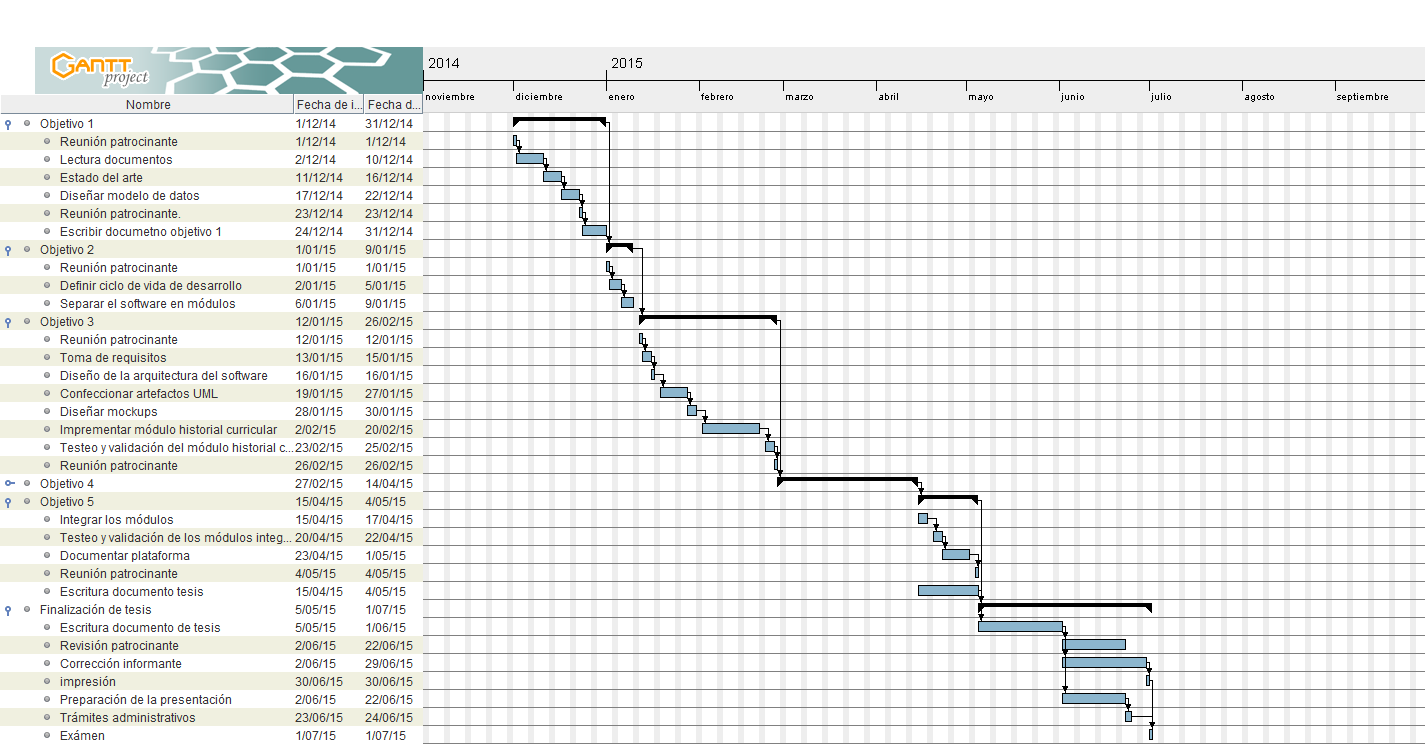
\includegraphics[width=1\textwidth]{images/Capitulo_3/carta_gantt.png}
		\caption[Carta Gantt que exhibe las etapas de desarrollo del sistema]{Carta Gantt que exhibe las etapas de desarrollo del sistema \footnote{}}
		\label{figura_cartaGantt}
	\end{figure}
	\footnotetext{Elaboración propia.}

	Durante el proceso de desarrollo del producto software es importante tener en cuenta lo siguiente:
	\begin{itemize}
		\item Es importante reunirse con el profesor patrocinante al comienzo, durante y al
		término de una iteración, para así aclarar y resolver requerimientos específicos del
		sistema que puedan surgir.
		\item El producto final se dará terminado cuando se hayan cumplido todos los requisitos
		del sistema.
	\end{itemize}

\subsection{Análisis}
	En esta sección se describen los requerimientos y casos de uso más representativos de cada módulo, los cuales fueron obtenidos y discutidos mediante  reuniones con el profesor patrocinador, con el objetivo de identificar los requisitos funcionales y no funcionales que deberían satisfacer el producto software final.
		
	\subsubsection{Requerimientos}
	A continuación se presenta una lista de los requisitos que se definieron para el producto software.

	\myparagraph{Requisitos funcionales}
	
	Los requisitos funcionales del sistema se presentan en la Tabla \ref{Tabla_requisitos_funcionales}.
	\\
	
	
	\begin{longtable}{l |p{11cm}}
	
		\caption{Requisitos funcionales}
		\label{Tabla_requisitos_funcionales}\\

		
		\hline
		\endfirsthead
		\multicolumn{2}{c}%
		{\tablename\ \thetable\ -- \textit{Continuación de la pagina anterior}} \\
		\hline
	
		\hline
		\endhead
		\hline \multicolumn{2}{r}{\textit{Continúa en la página siguiente}} \\
		\endfoot
		\hline
		\endlastfoot
		\rowcolor{LightBlue2} REQF-01 & Autentificación de usuario\\ \hline
		\textbf{Descripción} & El sistema debe ser capaz de diferenciar distintos tipos de usuarios, mediante el RUT, tipo de usuario y contraseña. Estos pueden ser de tres tipo: Administrador, Editor, y Subscriptor.\\ \hline \hline
		
		\rowcolor{LightBlue2} REQF-02 & Gestión de perfil\\ \hline
		\textbf{Descripción} & El sistema debe permitir que los usuarios puedan modificar su contraseña. Además  debe permitir que el Administrador pueda modificar los datos que el usuario ingresó al momento de registrarse.\\ \hline \hline
		
		\rowcolor{LightBlue2} REQF-03 & Desplegar historial curricular\\  \hline
		\textbf{Descripción} &El sistema debe permitir que  todos los usuarios  puedan ver el conjunto de hitos curriculares de una carrera en particular, mediante la facultad, la escuela y la carrera previamente ingresados por el usuario.\\ \\ \\
		\\  \hline \hline
		
		\rowcolor{LightBlue2} REQF-04 & Registro de usuarios\\ \hline
		\textbf{Descripción} & El sistema deberá permitir el registro de nuevos usuarios, los cuales deben ser creados por el Administrador. Los datos a solicitar son: RUT, nombre, apellido paterno, apellido materno, correo electrónico y rol. La contraseña será los 6 primeros dígitos del  RUT ingresado.\\ \hline
		
		\rowcolor{LightBlue2} REQF-05 & Gestión de documentos\\  \hline
		\textbf{Descripción} & El sistema debe permitir al Administrador y Editor crear nuevos registros curriculares, indicando el plan de estudio, la carrera y el tipo de hito: Modificación mayor, Modificación menor o Innovación Curricular, además  debe permitir subir uno o mas archivos en formato PDF por registros, los cuales el sistema los  tienen que clasificar en: Resolución, Comunicación Interna y Petición de requisitos.\\  \hline
		
		\rowcolor{LightBlue2} REQF-07 & Visor de PDF\\  \hline
		\textbf{Descripción} & El sistema debe permitir al usuario ver  cualquier documento que se encuentre almacenado en la base de datos.\\  \hline \hline
		
		
		\rowcolor{LightBlue2} REQF-08 & Notificaciones\\  \hline
		\textbf{Descripción} & El sistema desplegará distintos tipos de notificaciones al momento de realizar cualquier tipo de cambio (guardar, editar, eliminar). Los dos tipos de alertas que se consideraron en la plataforma web son : \textbf{Success} y \textbf{Error}. \\  \hline \hline
		
		\rowcolor{LightBlue2} REQF-09 & Almacenar bitácora de los usuarios\\  \hline
		\textbf{Descripción} & El sistema internamente debe almacenar todas las notificaciones de los eventos ocurridos en la plataforma a fin de tener un registro de  todas  las actividades  que realizan los usuarios en la plataforma. Un registro de la bitácora debe tener necesariamente esta compuesto por: Código de la alerta, mensaje de la alerta, fecha y el RUT de usuario quien ejecutó dicha alerta.\\  \hline
		
		\rowcolor{LightBlue2} REQF-10 & Visualización de bitácora\\  \hline
		\textbf{Descripción} & El sistema debe permitir al administrador visualizar todos los eventos ocurridos en el sistama.\\ 
	
	\end{longtable}

	\myparagraph{Requisitos no funcionales}
	Los requisitos no funcionales se presentan en la Tabla \ref{Tabla_requisitos_no_funcionales}.
	\\

	\begin{longtable}{l |p{11cm}}
		
		\caption{Requisitos no funcionales}
		\label{Tabla_requisitos_no_funcionales}\\
		
		
		\hline
		\endfirsthead
		\multicolumn{2}{c}%
		{\tablename\ \thetable\ -- \textit{Continuación de la pagina anterior}} \\
		\hline
		
		\hline
		\endhead
		\hline \multicolumn{2}{r}{\textit{Continúa en la página siguiente}} \\
		\endfoot
		\hline
		\endlastfoot
	
			\rowcolor{LightBlue2} REQNF-01 & Ambiente Web\\ \hline
			\textbf{Descripción} & El sistema debe visualizarse y funcionar correctamente en cualquier navegador, especialmente en Internet Explorer, Mozilla y Google Chrome.\\ \hline \hline
			
			\rowcolor{LightBlue2} REQNF-02 & Escalabilidad\\ \hline
			\textbf{Descripción} & El sistema debe estar en capacidad de permitir en el futuro el desarrollo de nuevas funcionalidades, modificar o eliminar funcionalidades.\\  \hline
			
			\rowcolor{LightBlue2} REQNF-03 & Facilidad de uso\\ \hline
			\textbf{Descripción} & La interfaz del sistema debe ser amigable con el usuario, Mensajes de errores y éxito.\\ \hline
			
	
			
			\rowcolor{LightBlue2} REQNF-04 & Facilidad de pruebas\\ \hline
			\textbf{Descripción} & El sistema debe contar con facilidad para la identificación de la localización de los errores durante la etapa de prueba.\\ \hline \hline
			
			\rowcolor{LightBlue2} REQNF-05 & Validación\\ \hline
			\textbf{Descripción} & El sistema tiene que poseer una interfaz en la cual se validen los campos obligatorios y  manejo de datos que se ingresan.\\ 
	\end{longtable}

	\subsubsection{Modelo conceptual}
	Para facilitar la compresión de la problemática que se desea solucionar mediante el producto software, en la Figura \ref{Figura_Modelo_conceptual}  se presenta un modelo conceptual, que muestra el dominio dentro del cual se encuentra inmerso el proyecto.
	\\
		\begin{figure}[H]
			\centering
			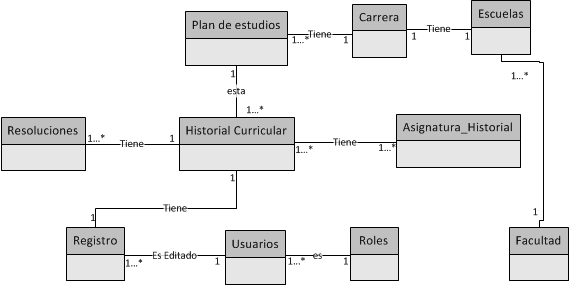
\includegraphics[width=1\textwidth]{images/Capitulo_3/Modelo_Conceptual.png}
			\caption[Modelo conceptual del proyecto]{Modelo conceptual del proyecto \footnote{}}
			\label{Figura_Modelo_conceptual}
		\end{figure}
		\footnotetext{Elaboración propia.}
	\subsubsection{Casos de uso}
	En las Figuras \ref{caso_uso_Administrador}, \ref{caso_uso_Editor}, \ref{caso_uso_Suscriptor} se presentan los diferentes casos de uso para los actores
	involucrados en el sistema.
	
	
	\begin{figure}[H]
		\centering
		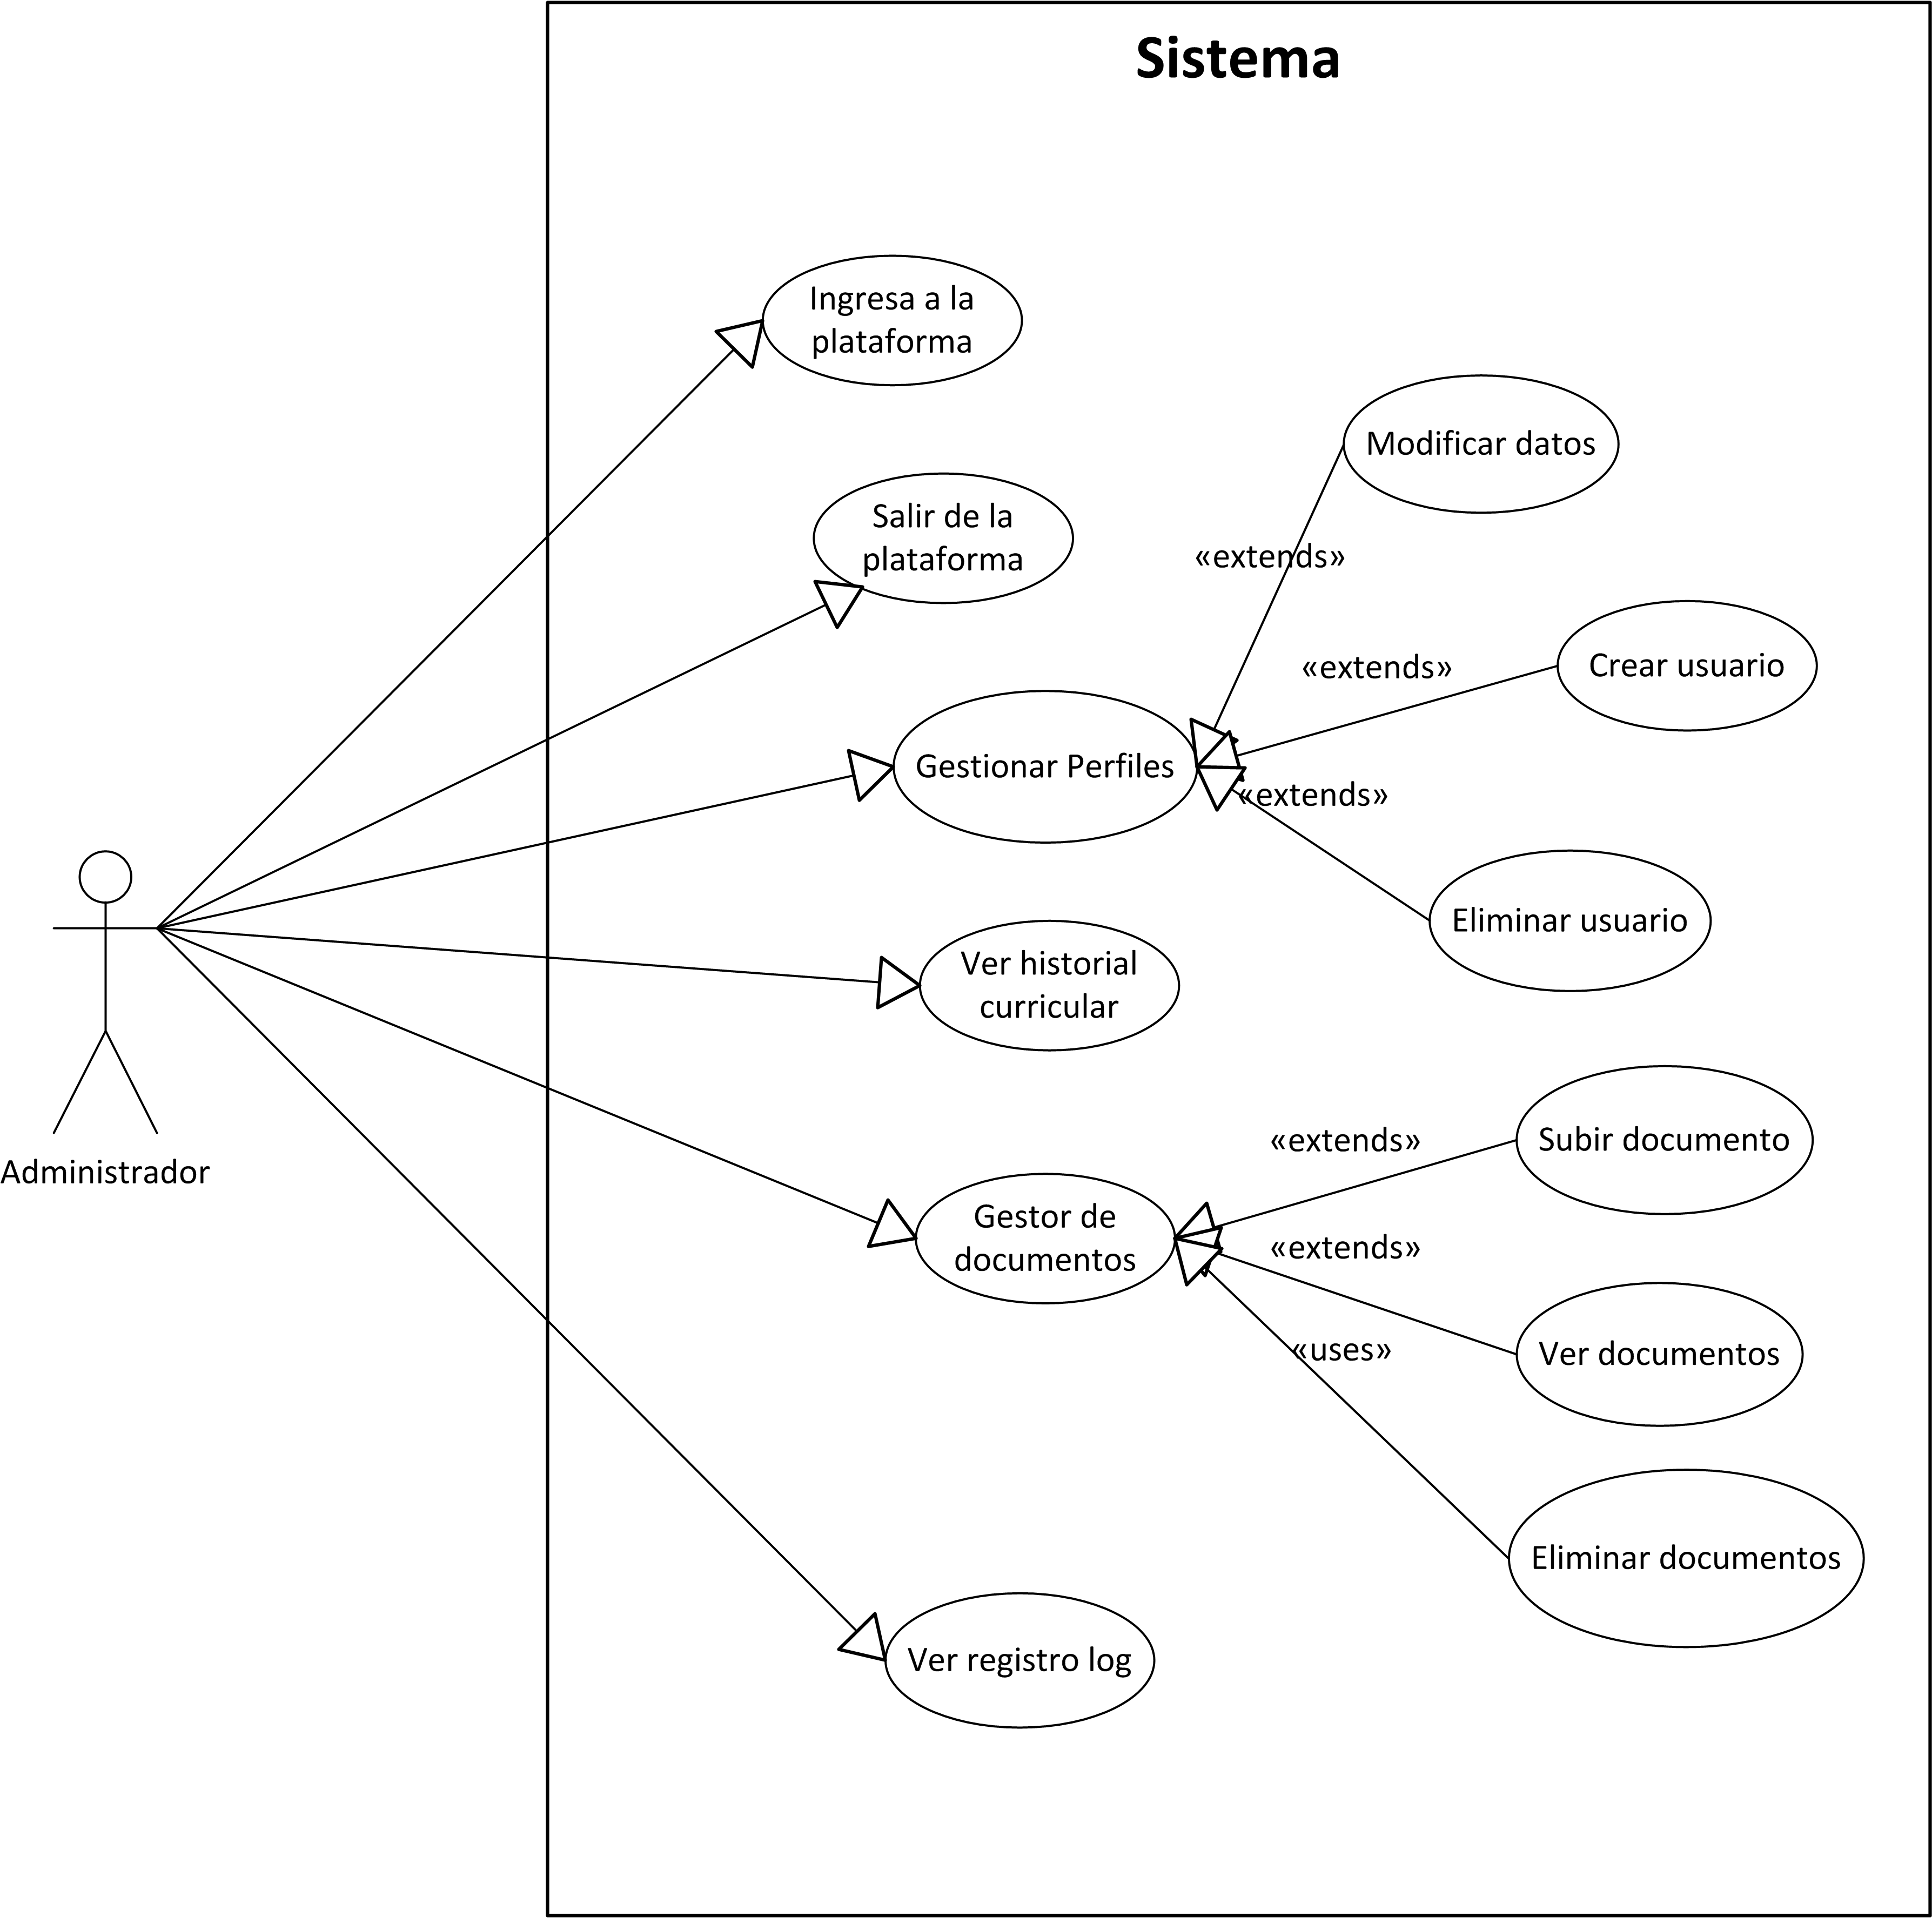
\includegraphics[width=1\textwidth]{images/Capitulo_3/caso_uso_Administrador.png}
		\caption[Diagrama de caso de uso para el Administrador]{Diagrama de caso de uso para el Administrador \footnote{}}
		\label{caso_uso_Administrador}
	\end{figure}
	\footnotetext{Elaboración propia.}
	
	\begin{figure}[H]
		\centering
		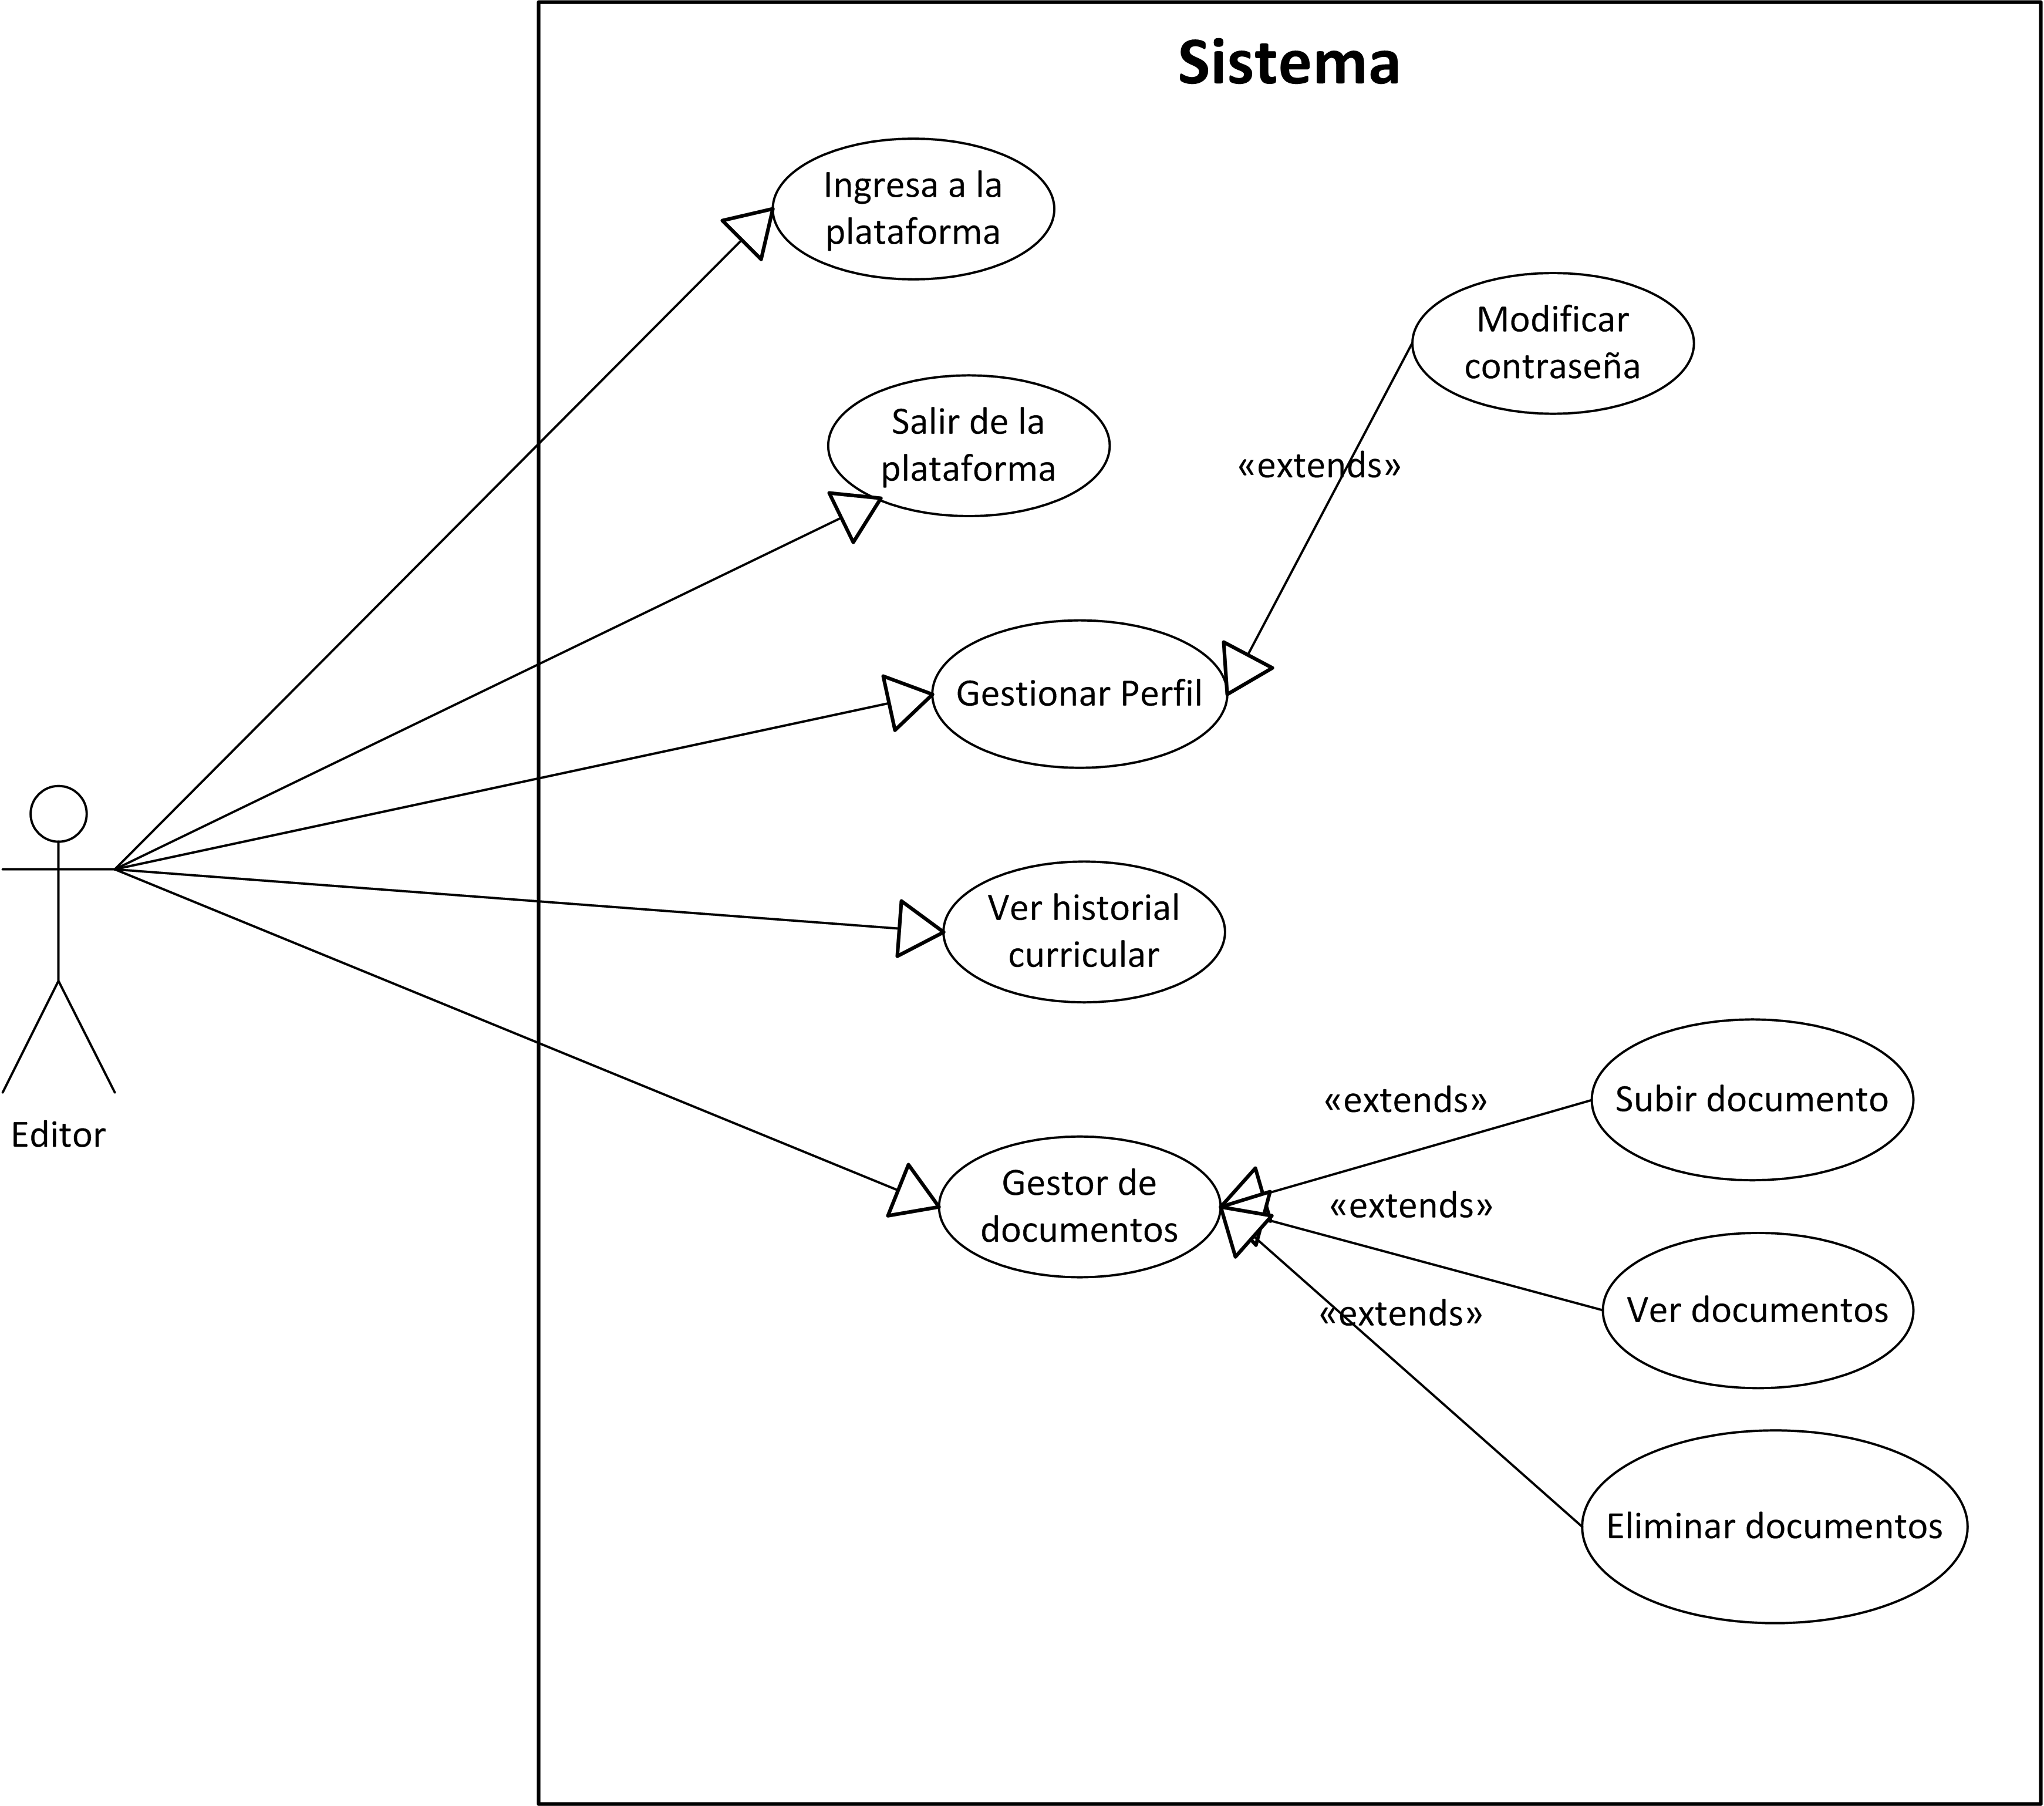
\includegraphics[width=1\textwidth]{images/Capitulo_3/caso_uso_Editor.png}
		\caption[Diagrama de caso de uso para el Editor]{Diagrama de caso de uso para el Editor \footnote{}}
		\label{caso_uso_Editor}
	\end{figure}
	\footnotetext{Elaboración propia.}
	
	\begin{figure}[H]
		\centering
		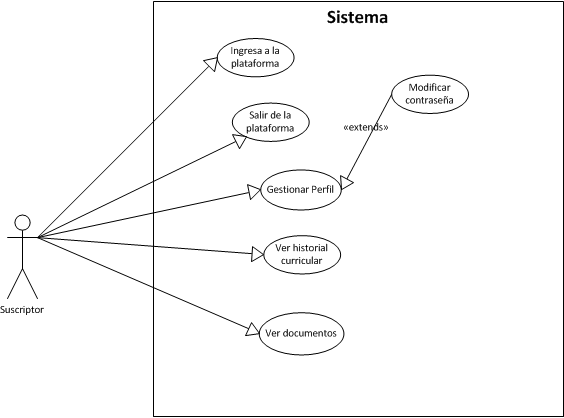
\includegraphics[width=1\textwidth]{images/Capitulo_3/caso_uso_Suscriptor.png}
		\caption[Diagrama de caso de uso para el Suscriptor]{Diagrama de caso de uso para el Suscriptor \footnote{}}
		\label{caso_uso_Suscriptor}
	\end{figure}
	\footnotetext{Elaboración propia.}
	
	\myparagraph{Descripción de los actores del sistema} \label{usuarios_Sistema}
	
	
	\textbf{Suscriptor:} corresponde al grupo de individuos que pueden revisar los datos en la plataforma, es decir, pueden ver el historial curricular de una carrera y ver todas las resoluciones. sin embargo no posee ningún permiso de edición o creación.
	\\
	
	\textbf{Editor:} Este grupo de individuos posee todos los permisos necesarios para poder realizar todas las operaciones básicas (crear, leer,editar y borrar) sobre los registros curriculares y/o los documentos que están en el sistema.
	\\
	
	\textbf{Administrador:} Corresponde al individuo o grupo de individuos que tiene todas las
	funciones de un creador de registros curriculares, pero que además es el encargado de administrar la
	totalidad de usuarios de la plataforma, lo cual incluye el registro, edición y eliminación
	de usuarios.
	
	
	
\subsection{Diseño e implementación}

	En esta sección se describe el diseño y la implementación para los módulos: \textit{Historial curricular} y \textit{Gestor de documentos} de la plataforma. En un principio se muestran algunos artefactos generales correspondientes al diagrama de componentes y al modelo de datos. Posteriormente para cada módulo se presentaran los casos de uso, además del diagrama de secuencia correspondiente.


	\subsubsection{Diagramas de componentes}
	
	En la Figura \ref{diagrama_Componente_SW} y \ref{diagrama_Componente_HW} se muestran los diagramas de componentes software y hardware respectivamente. Ambos diagramas son congruentes con lo visto en el Capítulo \ref{PseudoMVC}, correspondiente al patrón de diseño de programación que utiliza ASP.NET.
			\begin{figure}[H]
				\centering
				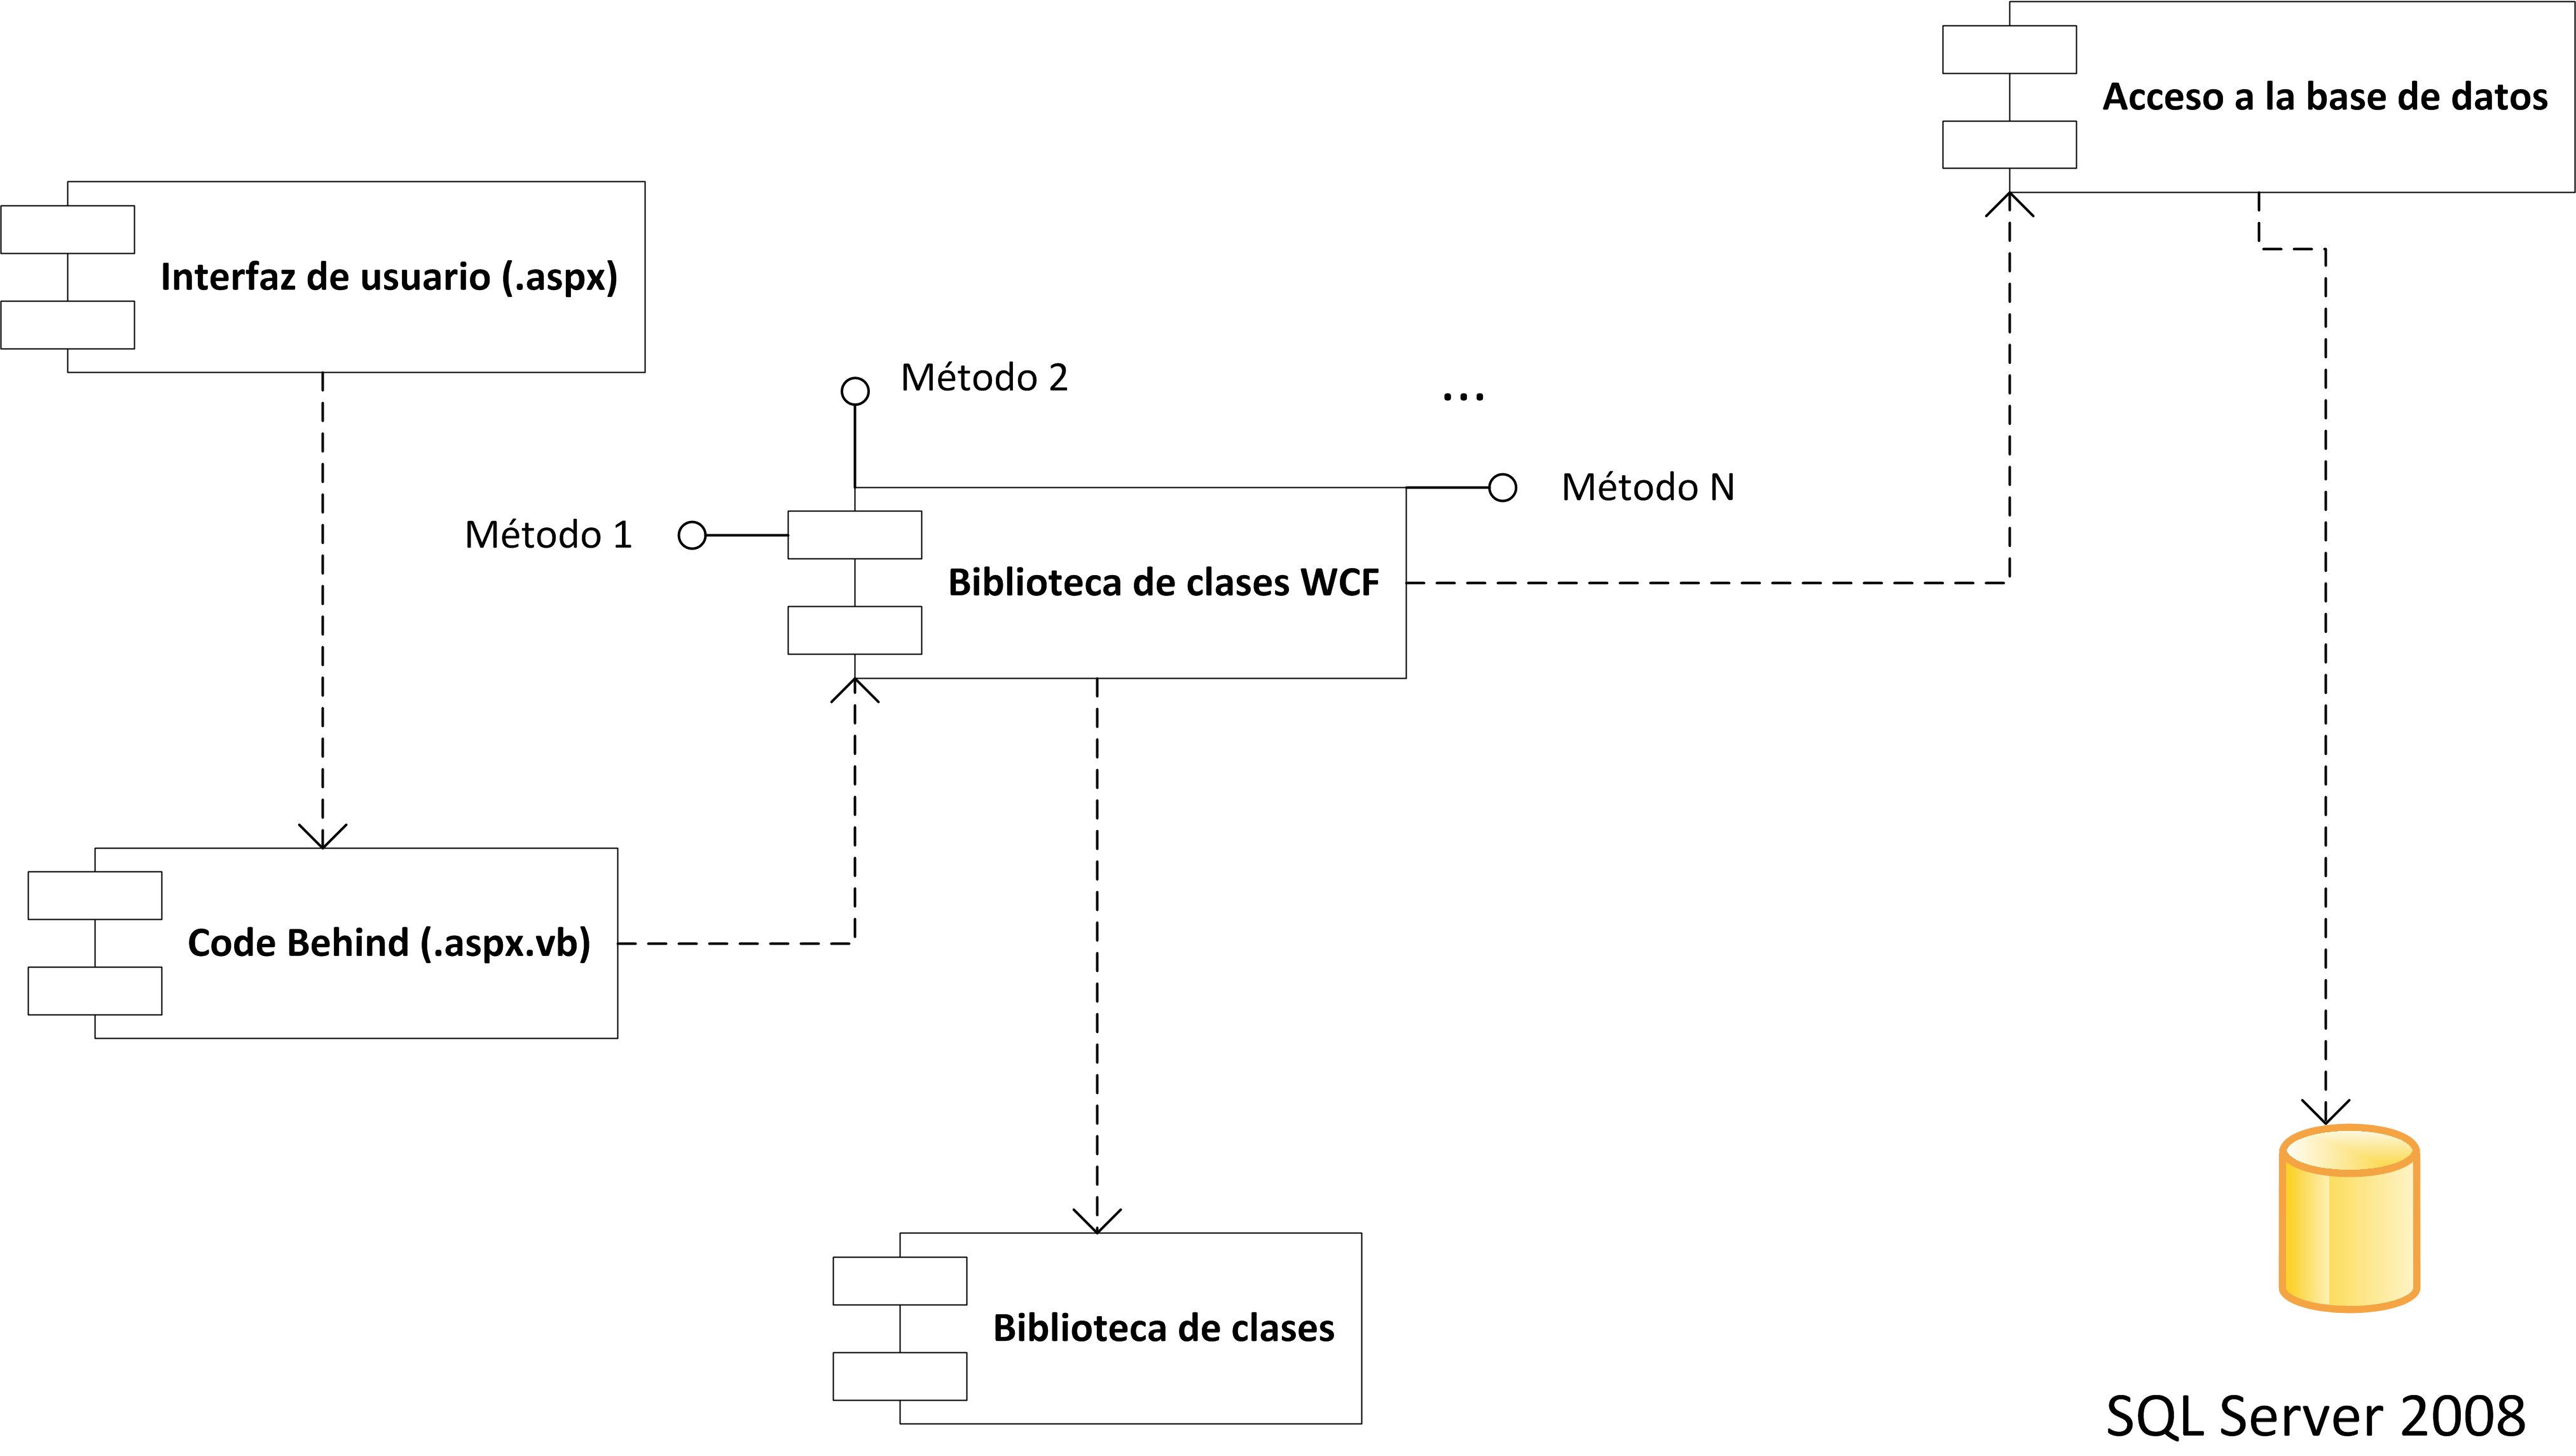
\includegraphics[width=1\textwidth]{images/Capitulo_3/Componente_SW.png}
				\caption[Diagrama de componentes Software del sistema]{Diagrama de componentes Software del sistema\footnote{}}
				\label{diagrama_Componente_SW}
			\end{figure}
			\footnotetext{Elaboración propia.}
	\begin{itemize}
		\item \textbf{Interfaz de usuario:} La interfaz de usuario  consta de los archivos aspx, los cuales no solo definen la estructura de las páginas en el sistema sino también  es el encargado de llamar todos los archivos CSS y JS necesarios para el correcto funcionamiento.
		
		
		\item \textbf{Code Behind:} Como se mencionó en la Sección \ref{ASP.NET}, ASP.NET permite organizar  los eventos  en forma separada de la interfaz. Todo lo relacionado con Interfaz de usuario se maneja en el archivo .aspx y el control de los eventos en un archivo separado .aspx.vb.
		
		\item \textbf{biblioteca de clases WCF:} Este componente contiene los servicios web de la aplicación.
		
		\item \textbf{biblioteca de clases:} Conjunto de clases que definen las estructuras de las  entidades de la base de datos.
		
		\item \textbf{Acceso a la base de datos:} El acceso a la base de datos se realiza  mediante un DLL que fue facilitado por la DTI.
	\end{itemize}		
			
		\begin{figure}[H]
			\centering
			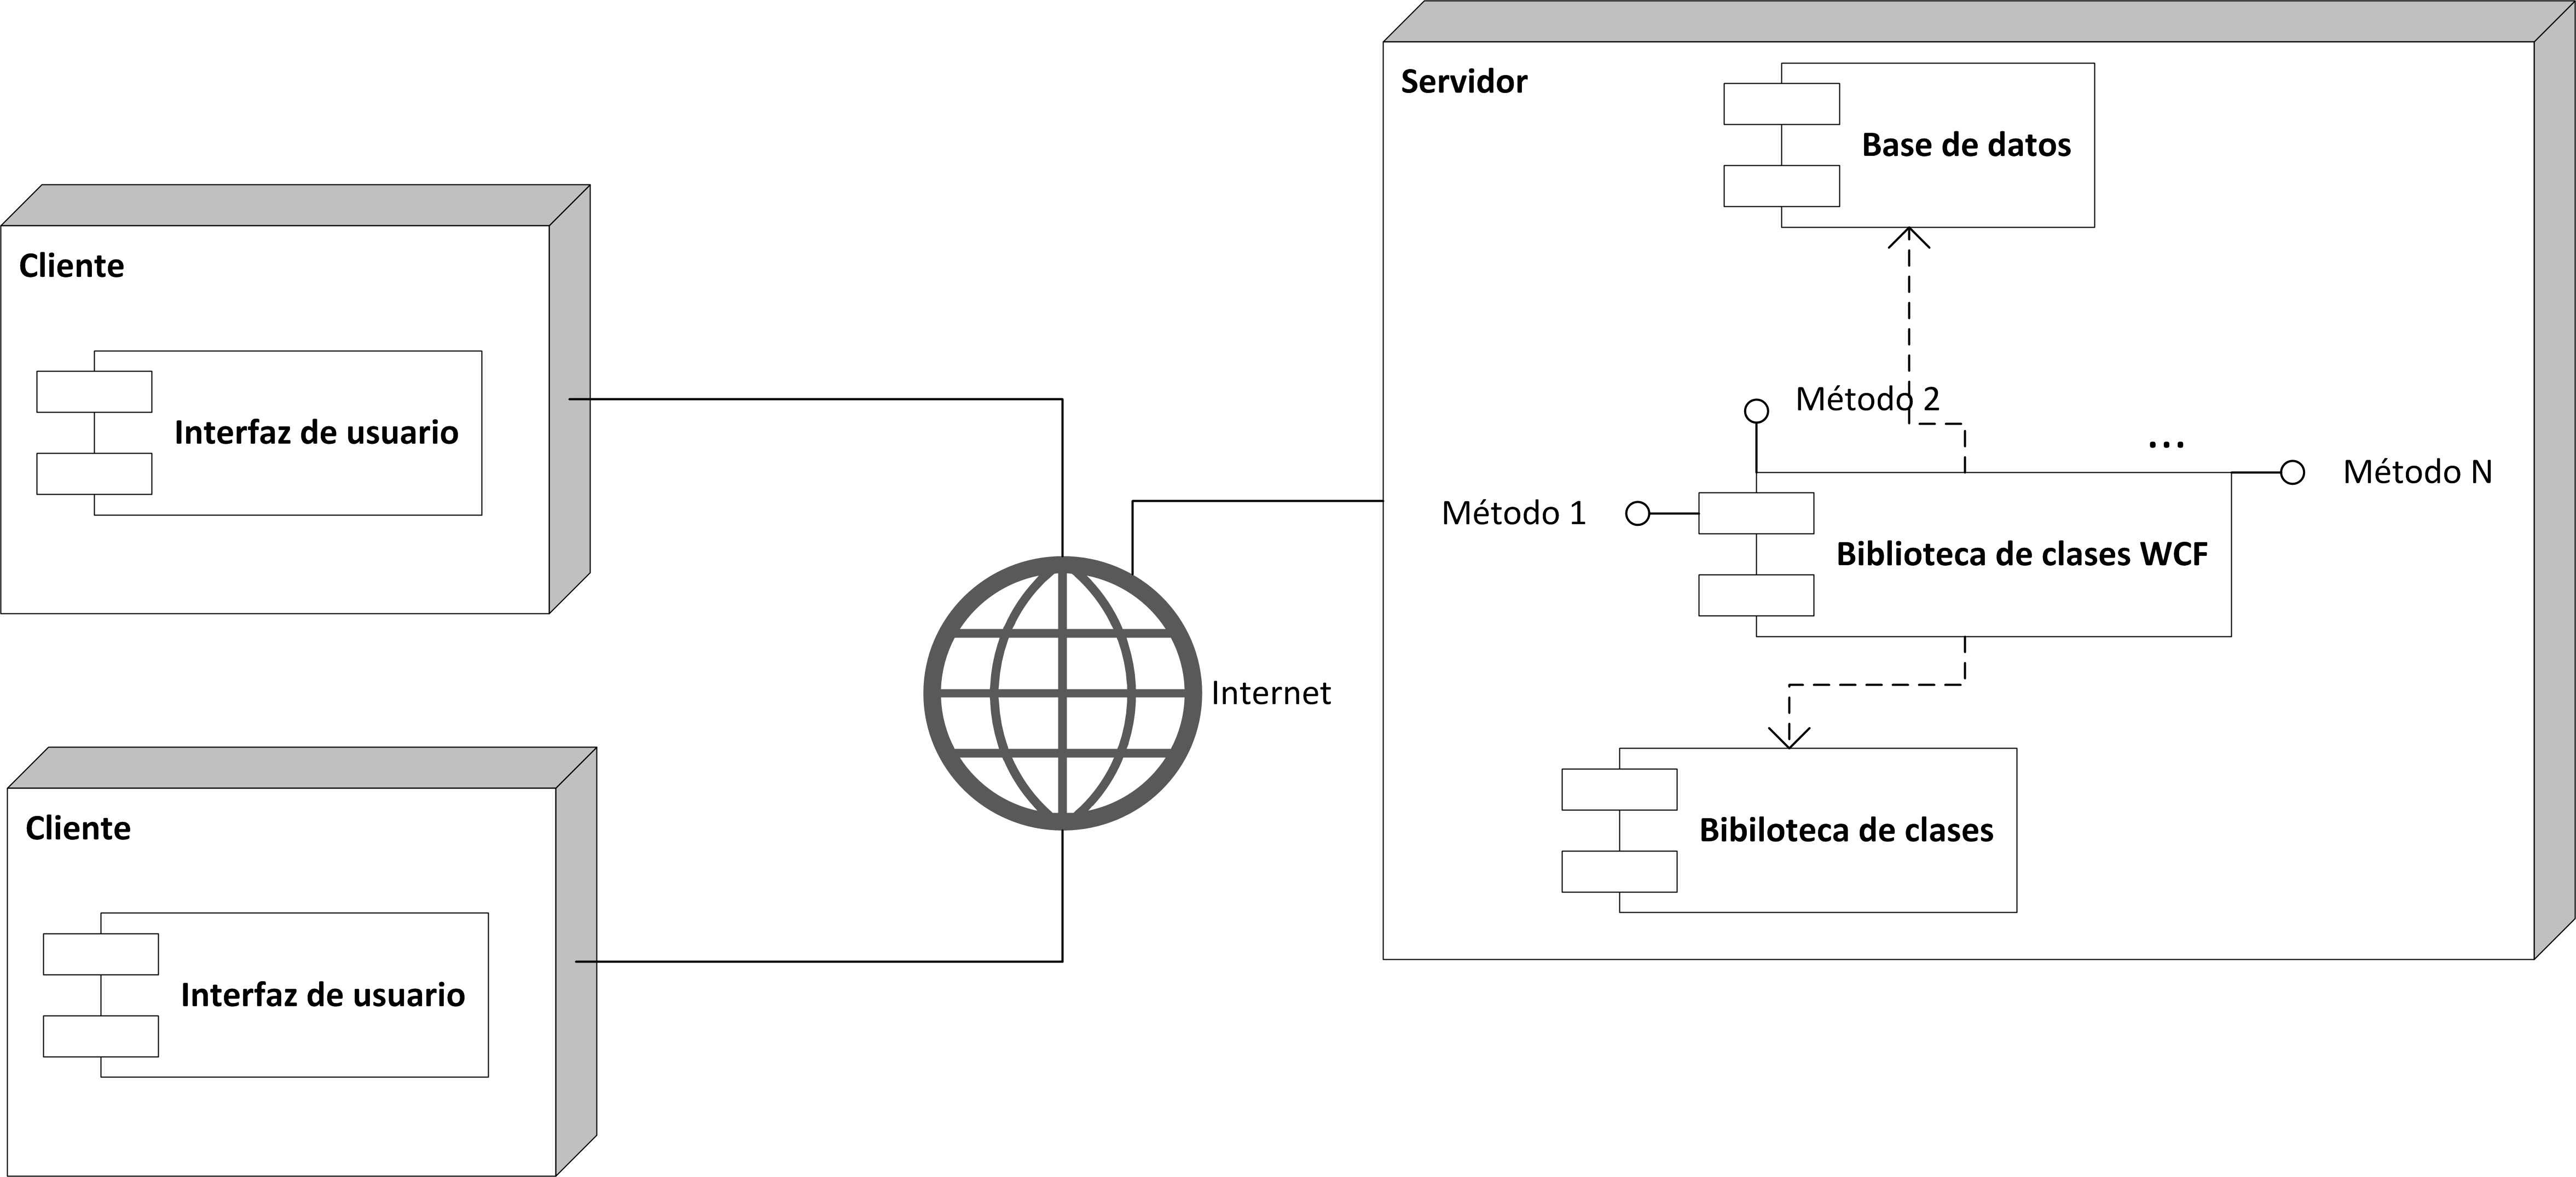
\includegraphics[width=1\textwidth]{images/Capitulo_3/Componente_HW.png}
			\caption[Diagrama de componentes Hardware del sistema]{Diagrama de componentes Hardware del sistema\footnote{}}
			\label{diagrama_Componente_HW}
		\end{figure}
		\footnotetext{Elaboración propia.}
		
	\subsubsection{Modelo de datos}
	
	El contexto en el que se desenvuelve el software contempla 14 entidades, de las cuales 8 de ellas se exportaron desde la base de datos de la Universidad para poder trabajar en un ambiente de desarrollo, estas entidades son: Facultad, Escuelas, Carreras, PlanEstudio, PlanAsignatura, Plan\_asig\_requisito,institutos y asignaturas.
	\\
	
	Las entidades restantes fueron creadas con el fin de satisfacer las necesidades de la problemática en la cual se encuentra inmerso en proyecto. El modelo de datos completo se puede ver en la Figura \ref{Modelo_E_R}.
	\\
	
	\begin{figure}[H]
		\centering
		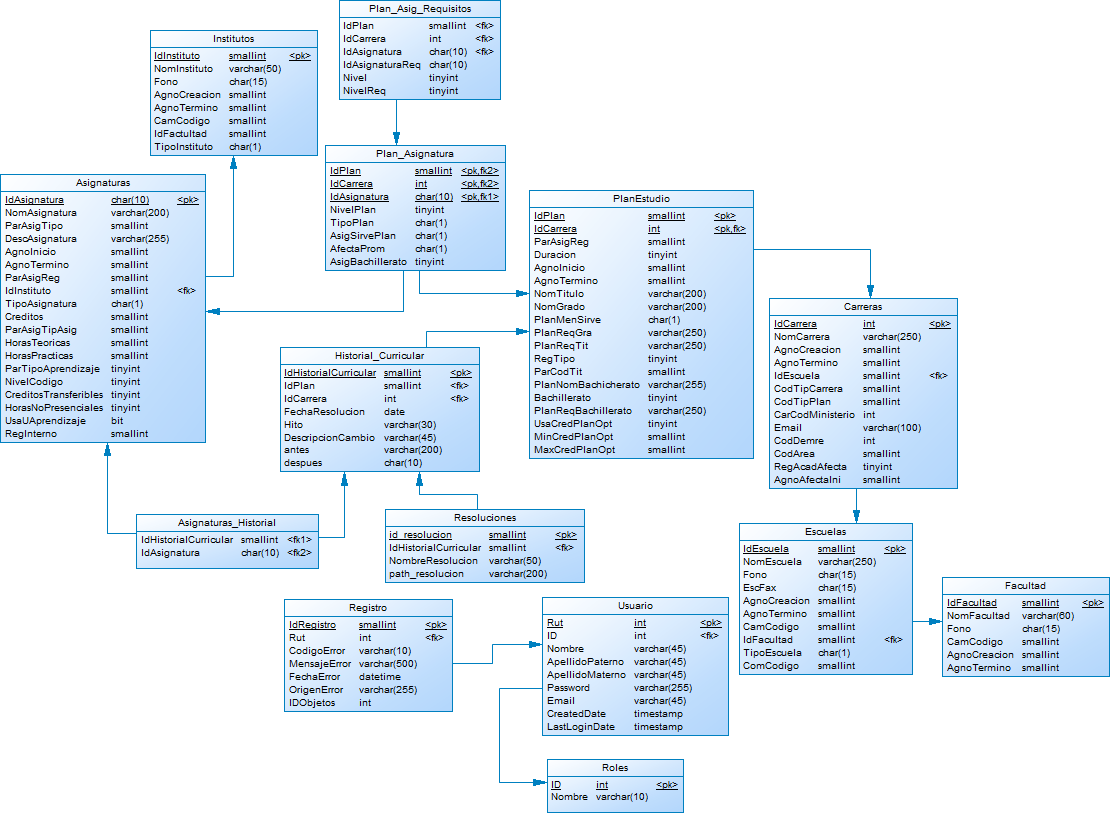
\includegraphics[width=1\textwidth]{images/Capitulo_3/Modelo_E_R.png}
		\caption[Modelo de datos Entidad-Relación]{Modelo de datos Entidad-Relación \footnote{}}
		\label{Modelo_E_R}
	\end{figure}
	\footnotetext{Elaboración propia.}
	
	\myparagraph{Diccionario de datos}
	
	Es importante que todo proyecto el cual involucre un almacenamiento de datos, posea un diccionario de datos, puesto que el  objetivo de un diccionario de datos  es dar precisión sobre los datos	que se manejan en un sistema, evitando así  malas interpretaciones.
	\\
	
	Como se mencionó anteriormente, no todas las entidades son de creación propia, por lo que el en Anexo C se puede ver el diccionario de datos correspondiente solo a las tablas creadas.
	
	
	
	\subsubsection{Módulo historial curricular}
	
	El módulo historial curricular esta diseñado para que todos los usuarios definidos en la Sección \ref{usuarios_Sistema} tengan acceso a él, a causa de que su principal objetivo es ver la trazabilidad de una carrera en particular.
	\myparagraph{Diseño}
	A continuación se describe el diseño del caso de uso más significativo para el módulo  historial curricular de la plataforma, que corresponde a la visualización de la trazabilidad de los planes de estudio de las carreras . Se presentará en detalle la composición de este caso de uso y su participación en el sistema.
		
	\mysubparagraph{ Caso de uso real más significativo} 
	
	El caso de uso “Ver historial curricular” ocurre cuando un usuario  desea  ver los cambios  curriculares que se le han aplicado a una carrera en particular. El caso de uso real “Ver historial curricular” se presenta en la Tabla \ref{Tabla_Caso_Uso_ver_historial}.
	
	
		\begin{longtable}{p{7cm}| p{7cm}}
			
			\caption{Caso de uso Ver historial curricular}
			\label{Tabla_Caso_Uso_ver_historial}\\
			
			
			\hline
			\endfirsthead
			\multicolumn{2}{c}%
			{\tablename\ \thetable\ -- \textit{Continuación de la página anterior}} \\
			\hline
			
			\hline
			\endhead
			\hline \multicolumn{2}{r}{\textit{Continúa en la página siguiente}} \\
			\endfoot
			\hline \hline
			\endlastfoot
			\rowcolor{LightBlue2}  \multicolumn{2}{c}{Caso de Uso Ver Historial Curricular} \\  \hline
			
			
			\textbf{Actores} & Administrador, Editor, Suscriptor.\\ \hline
			
			\textbf{Propósito} & Visualizar los cambios curriculares que se han realizado en una determinada carrera.\\ \hline
			
			\textbf{Tipo} & Primario y esencial\\ \hline
			
			\multicolumn{2}{p{15cm}}{\textbf{Resumen:} Un usuario autentificado puede ver el historial curricular de una carrera en particular, el cual lo hace primero seleccionado la facultad a la que pertenece, luego la escuela y por último selecciona la carrera en cuestión.} \\  \hline \hline
			 
			\rowcolor{LightBlue2}  \multicolumn{2}{c}{Interfaz: Formulario Ver Historial Curricular} \\  \hline \hline
			
			\multicolumn{2}{c}{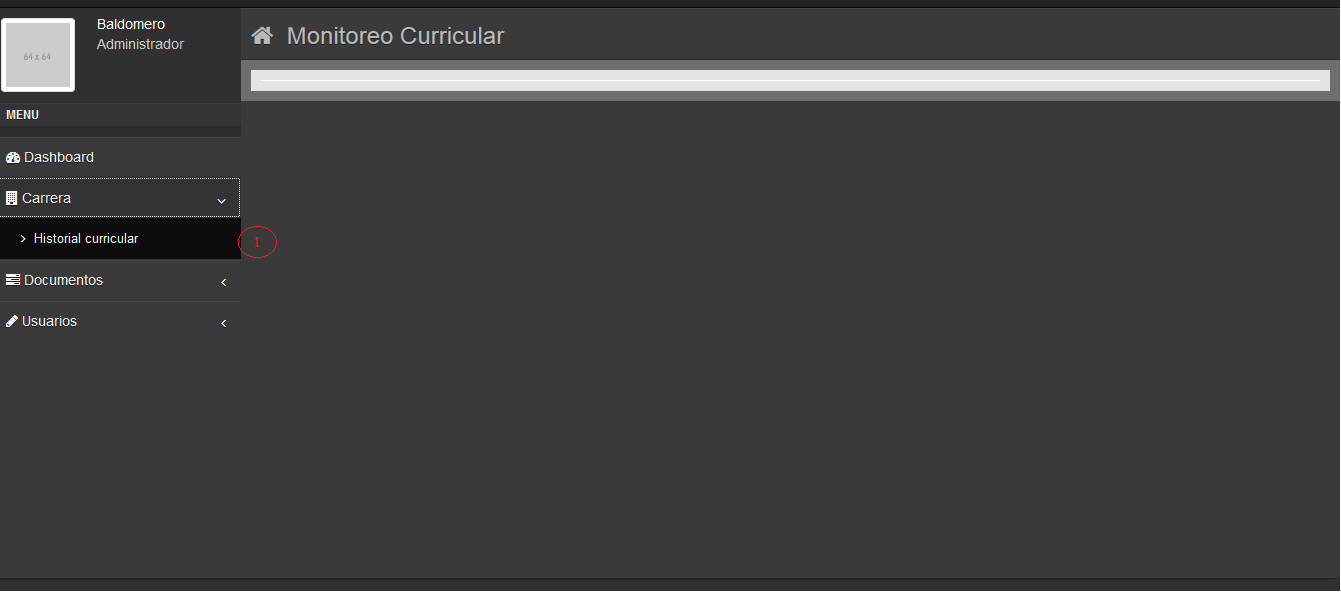
\includegraphics[width=1\textwidth]{images/Capitulo_3/F_historialCurricular1.png}} \\ 
			
			\multicolumn{2}{c}{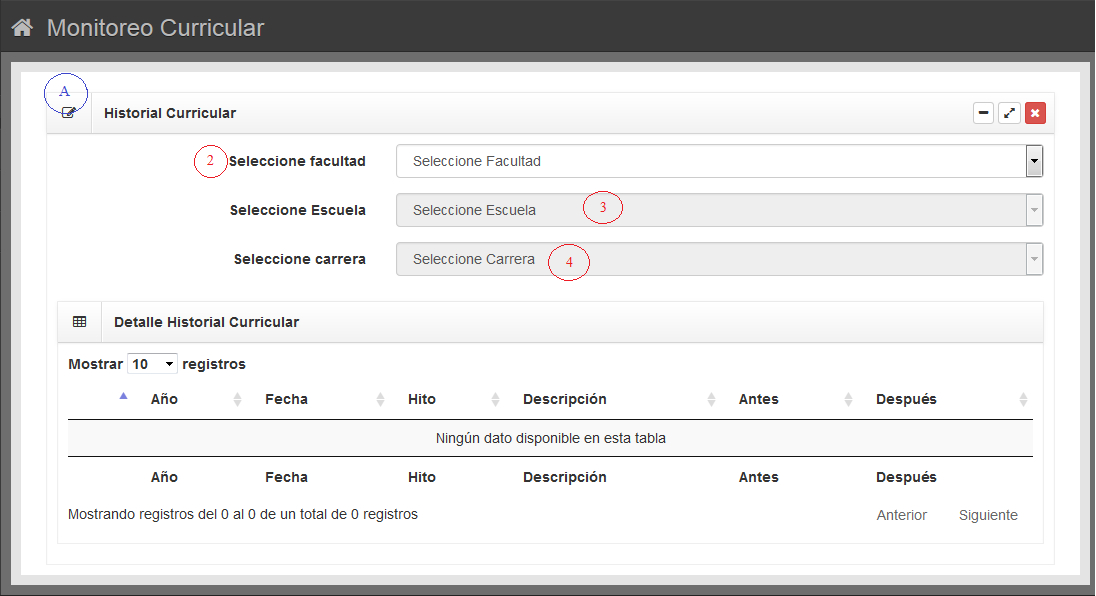
\includegraphics[width=1\textwidth]{images/Capitulo_3/F_historialCurricular2.png}} \\ 
			
			\multicolumn{2}{c}{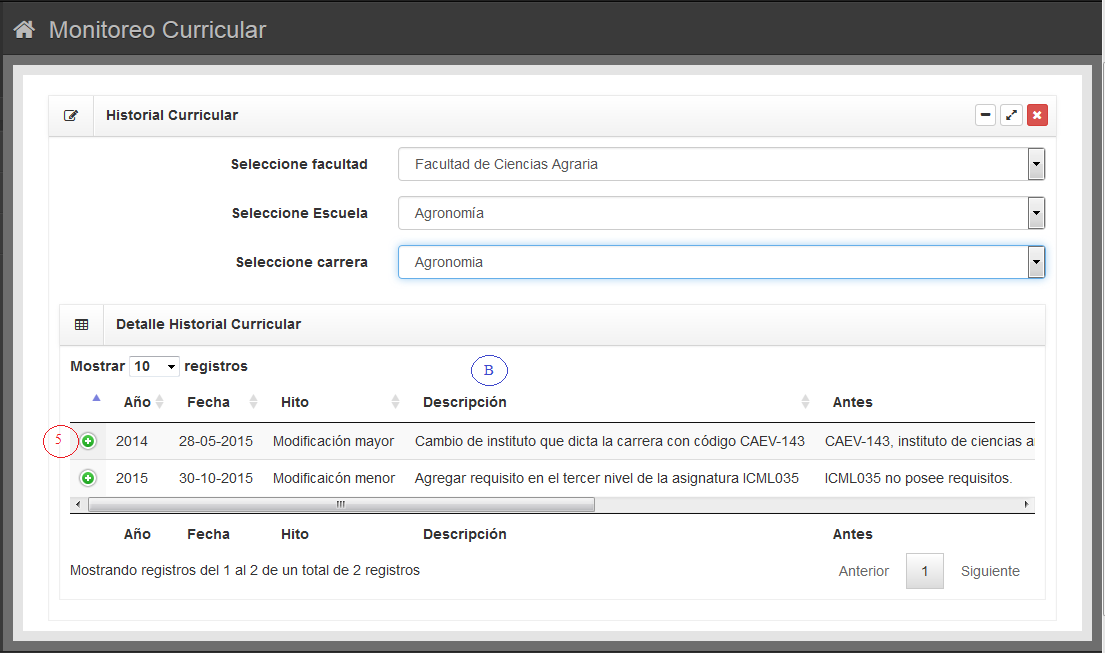
\includegraphics[width=1\textwidth]{images/Capitulo_3/F_historialCurricular3.png}} \\ 
			
			\multicolumn{2}{c}{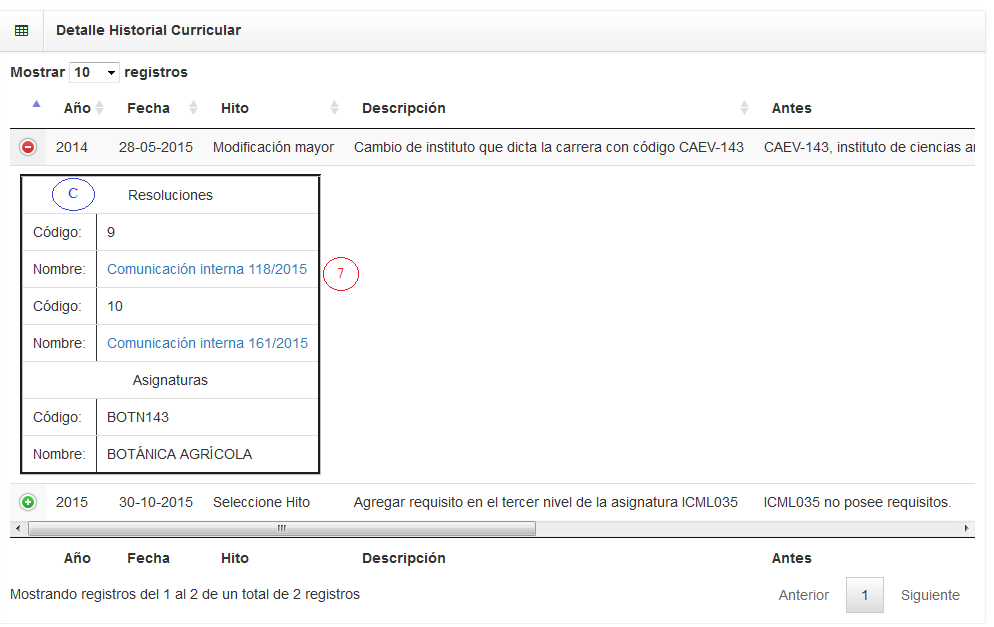
\includegraphics[width=1\textwidth]{images/Capitulo_3/F_historialCurricular4.png}} \\ \hline
			
			\rowcolor{LightBlue2}  \multicolumn{2}{c}{Curso normal de eventos} \\ 
			
			\textbf{Acción actor} &	\textbf{Respuesta sistema} \\ \hline
			
			1.- Este caso de uso comienza cuando un usuario autentificado desea ver el historial curricular de una carrera, para ello debe hacer click en \textbf{1}.
			 &	2.- El sistema despliega la pantalla \textbf{A}, el cual permite al usuario seleccionar facultad, escuela y carrera. \\ \hline
		
		
			3.- El usuario selecciona la facultad, escuela y carrera, haciendo click en \textbf{2},\textbf{3} y \textbf{4}.
			&	4.- El sistema crear un texto plano en formato JSON, el cual contiene el detalle solicitado por el usuario.\\ \hline
			
			
			& 5.- El sistema lee el archivo JSON y lo despliega en la tabla \textbf{B}.\\ \hline
			
			6.- Para ver información mas detallada del hito, el usuario puede hacer click en \textbf{6}.
			&	7.- El sistema despliega la información solicitada en \textbf{C}.\\ \hline
		
		
			8.- Si el usuario lo desea, puede ver la resolución haciendo click en \textbf{7}.
			&	9.- El sistema redirecciona al usuario al documento solicitado.\\ \hline
		\end{longtable}
		
		
		En la Figura \ref{diagrama_secuencial_ver_historial} se presenta el diagrama de secuencia para este mismo caso de uso, y así mostrar la interacción entre los distintos componentes del software que llevan a cabo esta tarea.
		
			\begin{figure}[H]
				\centering
				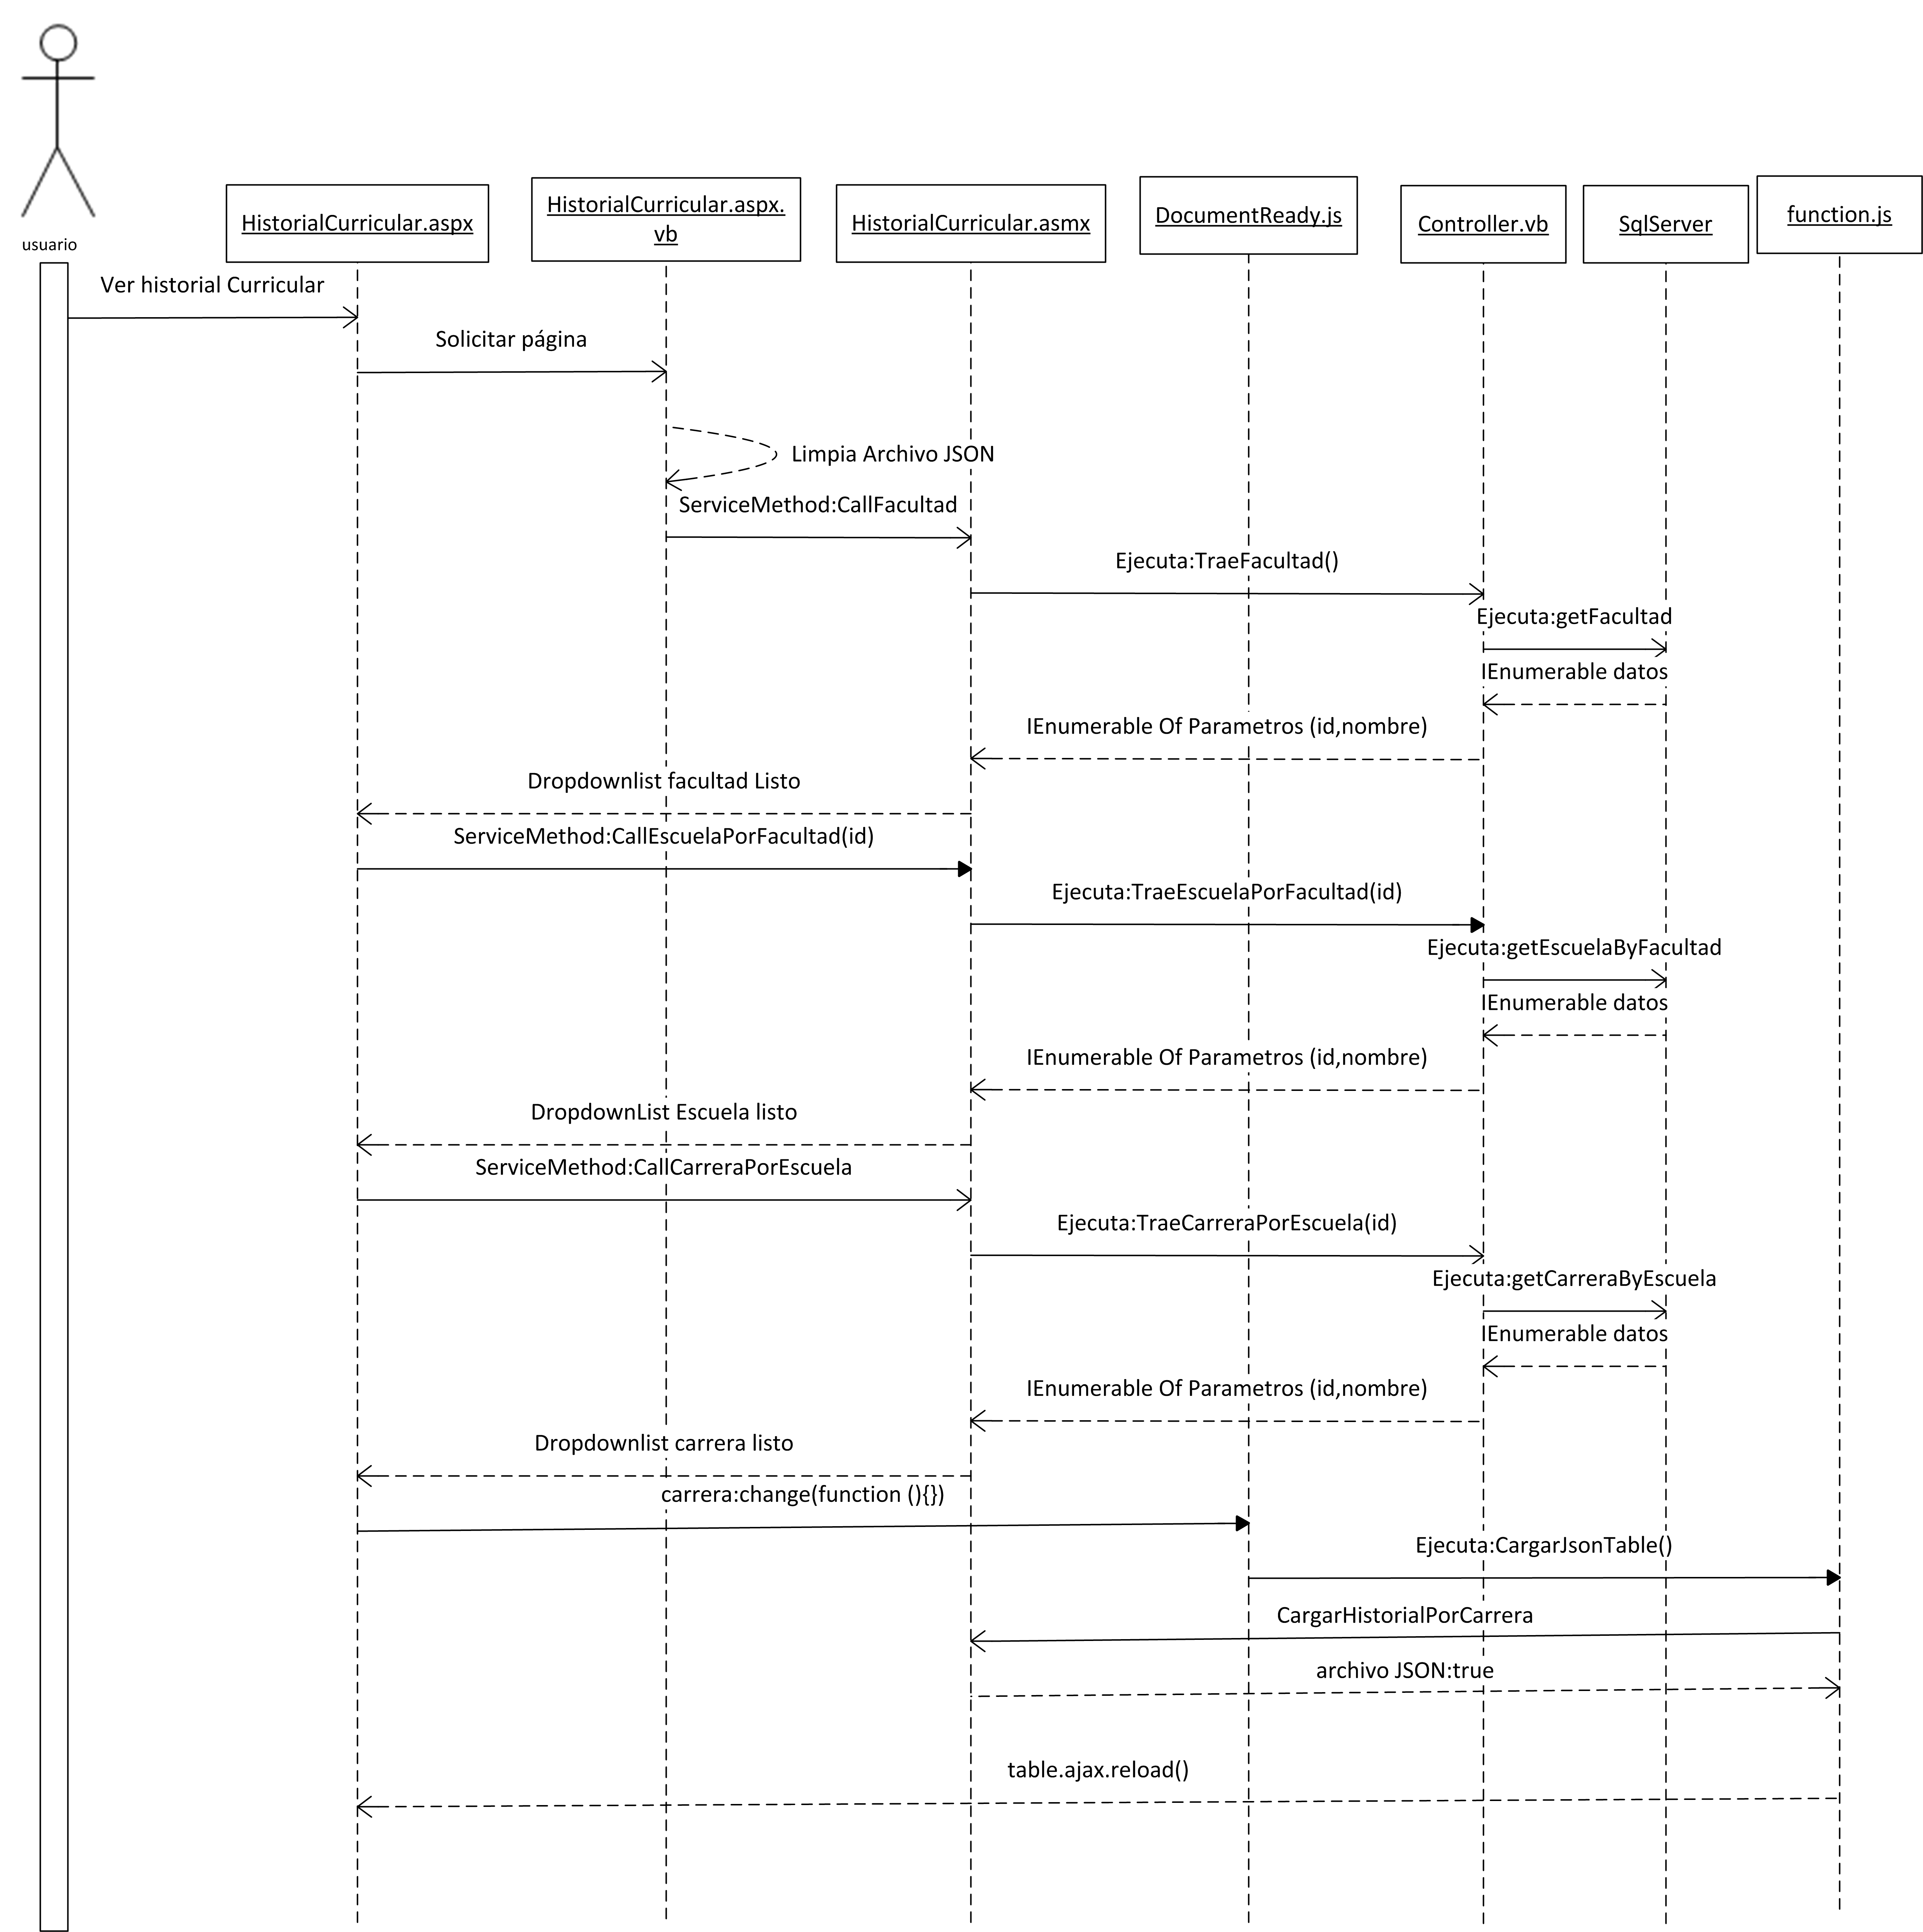
\includegraphics[width=1\textwidth]{images/Capitulo_3/diagrama_secuencial_Historial_Curricular.png}
				\caption[Diagrama de secuencia para el caso de uso \textit{Ver Historial Curricular}]{Diagrama de secuencia para el caso de uso \textit{Ver Historial Curricular} \footnote{}}
				\label{diagrama_secuencial_ver_historial}
			\end{figure}
			\footnotetext{Elaboración propia.}

		
		 En primer lugar el \textit{HistorialCurricular.aspx}  debe asegurarse que el archivo JSON de donde se leen los datos este vacío y con el formato adecuado para su correcta lectura(el formato del arhivo JSON utilizado se puede ver en el Anexo A). Una vez realizada esta acción, la vista se comunica con el servicio web (HistorialCurricular.asmx) para que la primera lista desplegable, correspondiente a las facultades  de la universidad,  no este vacía.\\
		 
		  El proceso que se describirá a continuación es la secuencia de pasos que realiza el sistema para  ``poblar'' una lista desplegable, por lo que este proceso se repite tres veces, la única diferencia es quién activa el proceso. Para la lista desplegable que se llena con las facultades la activa el sistema antes de mostrar el formulario al usuario, mientras que para las listas desplegables que abarcan a las escuelas y a las carreras las activa el usuario al momento de producir un cambio en las listas desplegables de niveles superiores, es decir, 
		  para que  el sistema poble la lista desplegable que contiene a las escuelas, el usuario debe producir un cambio en el DropDownList que contiene a  las facultades, y para poblar el DropDownList que contiene a las carreras, el usuario debe producir un cambio en la lista desplegable que abarca a las escuelas.\\

		
		
	
		El   \textbf{poblado de una lista desplegable} comienza cuando el HistorialCurricular.asmx  envía un mensaje a  la  \label{Proceso_poblado_DDL} biblioteca Controller.vb indicando qué datos se necesitan de la base de datos (Facultad, Escuela o Carrera), una vez que el Controller.vb recibe la petición, ejecuta  la consulta correspondiente y  retorna los datos solicitados en formato IEnumerable al servicio web, con el fin de que éste último actor asigne la información retornada en la lista desplegable correspondiente.
		\\
		
	
		Una vez que  el sistema haya verificado el estado del archivo JSON y que haya poblado la lista desplegable de las facultades, la plataforma esta en condiciones de mostrar el formulario al usuario para su posterior manipulación.		Por otra parte el DocumentReady.js esta a la espera de que el usuario seleccione la carrera, a fin de enviar un mensaje al Function.js con el ID de la carrera.
		\\
		
		Una vez que el actor Function.js reciba el ID de la carrera,  lo envía al servicio web para que éste cree el archivo JSON, tan pronto como se cree el archivo el HistorialCurricular.asmx  envía la variable JSON=true al actor Function.js para que se visualicen los datos del archivo JSON en la interfaz web.
		
		\subsubsection{Módulo Gestor de Documentos}
	
	
		El  módulo Gestor de documentos permite al administrador y editor administrar el repositorio de documentos de la plataforma, dicho de otra manera, estos usuarios podrán: crear, leer, editar y eliminar registros. Con respecto al usuario de tipo suscriptor, solo poseerá permisos de lectura.
	
		\myparagraph{Diseño}
		
		A continuación se describe el diseño de los dos  casos de usos extendidos del módulo de gestión de documentos de la plataforma, que corresponden a: subir documentos y  ver documentos. Se presentará en detalle la composición de estos casos de uso y su participación en el sistema.
		
		\mysubparagraph{ Caso de uso real del módulo gestor de documentos:``Subir documento''} 
		




		El caso de uso ``Subir documento'' corresponde al caso de uso extendido de ``Gestor de documentos'' y  ocurre cuando un administrador o un editor desea crear algún hito curricular en un plan de estudios. El caso de uso real ``Subir documento'' se presenta en la Tabla \ref{Tabla_Caso_Uso_Subir_Documento}.
		
		
		
		
			\begin{longtable}{p{7cm}| p{7cm}}
				
				\caption{Caso de uso  Subir Documento}
				\label{Tabla_Caso_Uso_Subir_Documento}\\
				
				
				\hline
				\endfirsthead
				\multicolumn{2}{c}%
				{\tablename\ \thetable\ -- \textit{Continuación de la página anterior}} \\
				\hline
				
				\hline
				\endhead
				\hline \multicolumn{2}{r}{\textit{Continúa en la página siguiente}} \\
				\endfoot
				\hline \hline
				\endlastfoot
				\rowcolor{LightBlue2}  \multicolumn{2}{c}{Caso de uso  Subir Documento} \\  \hline
				
				
				\textbf{Actores} & Administrador y Editor.\\ \hline
				
				\textbf{Propósito} & Crear un hito curricular a un plan de estudios.\\ \hline
				
				\textbf{Tipo} & Primario y esencial\\ \hline
				
				\multicolumn{2}{p{15cm}}{\textbf{Resumen:} El objetivo de este módulo es hacer posible la creación de hitos curriculares y la carga de documentos relacionados con el hito en cuestión al servidor.} \\  \hline \hline
				
				\rowcolor{LightBlue2}  \multicolumn{2}{c}{Interfaz: Formulario Ver Historial Curricular} \\  \hline \hline
				
				\multicolumn{2}{c}{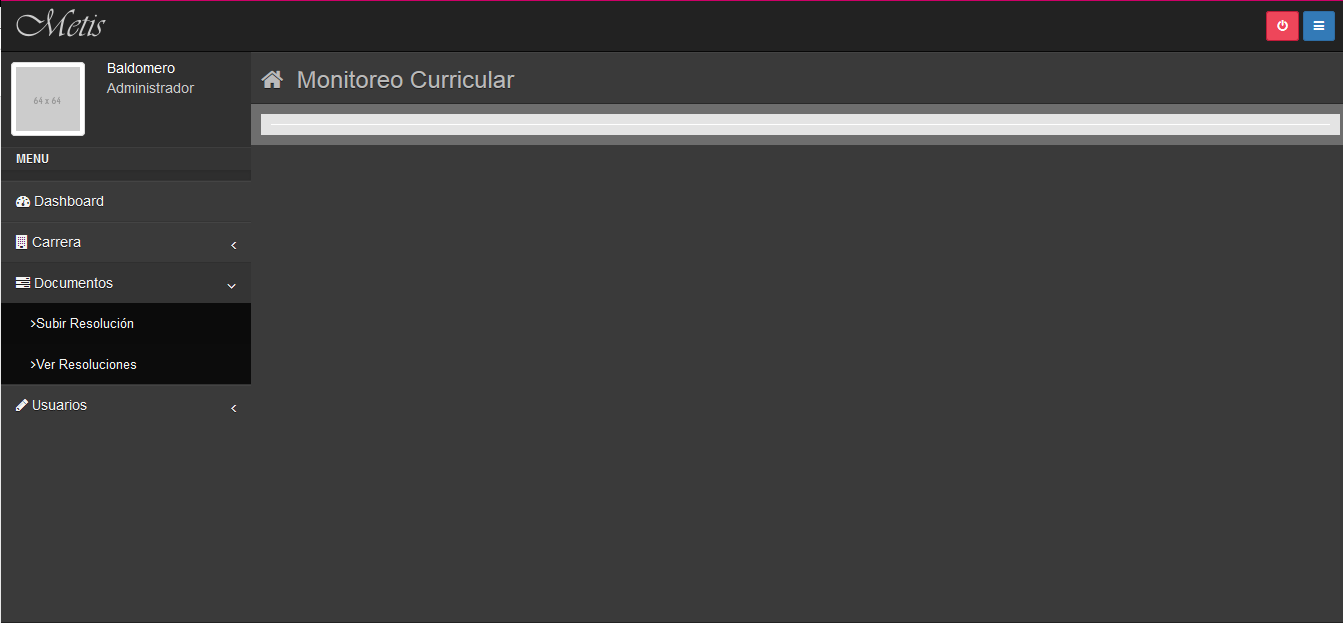
\includegraphics[width=1\textwidth]{images/Capitulo_3/subir_documento1.png}} \\ 
				
				\multicolumn{2}{c}{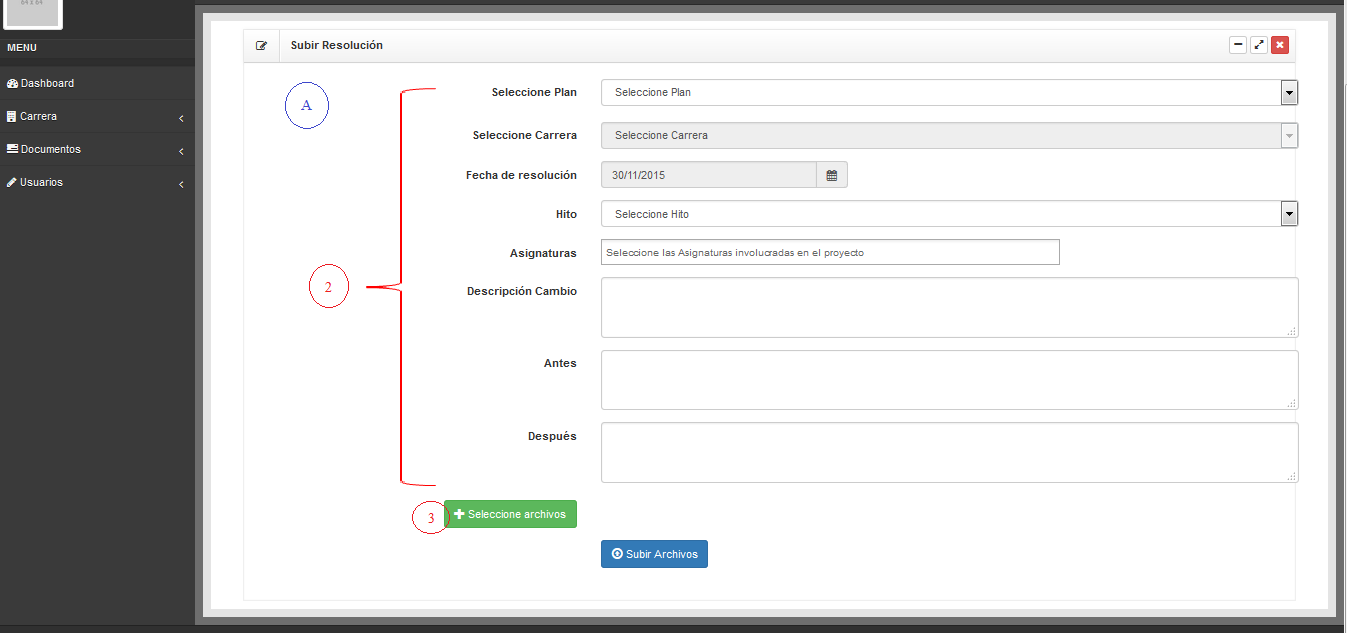
\includegraphics[width=1\textwidth]{images/Capitulo_3/subir_documento2.png}} \\ 
				
				\multicolumn{2}{c}{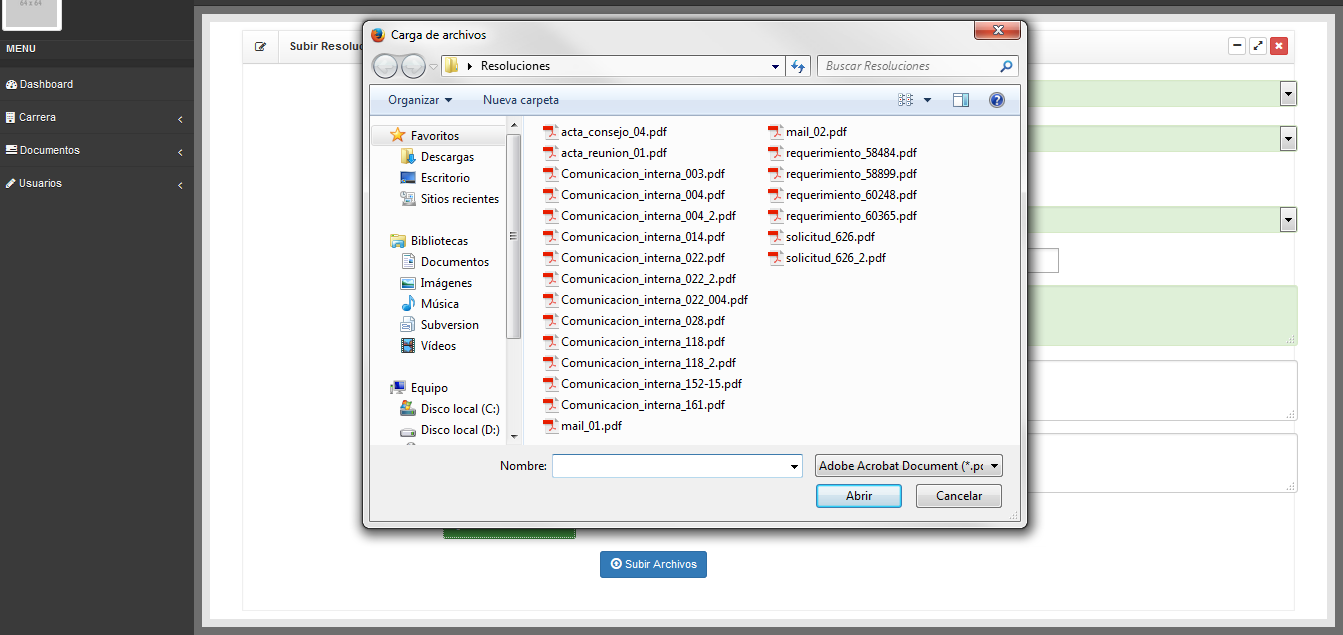
\includegraphics[width=1\textwidth]{images/Capitulo_3/subir_documento3.png}} \\ 
				
				\multicolumn{2}{c}{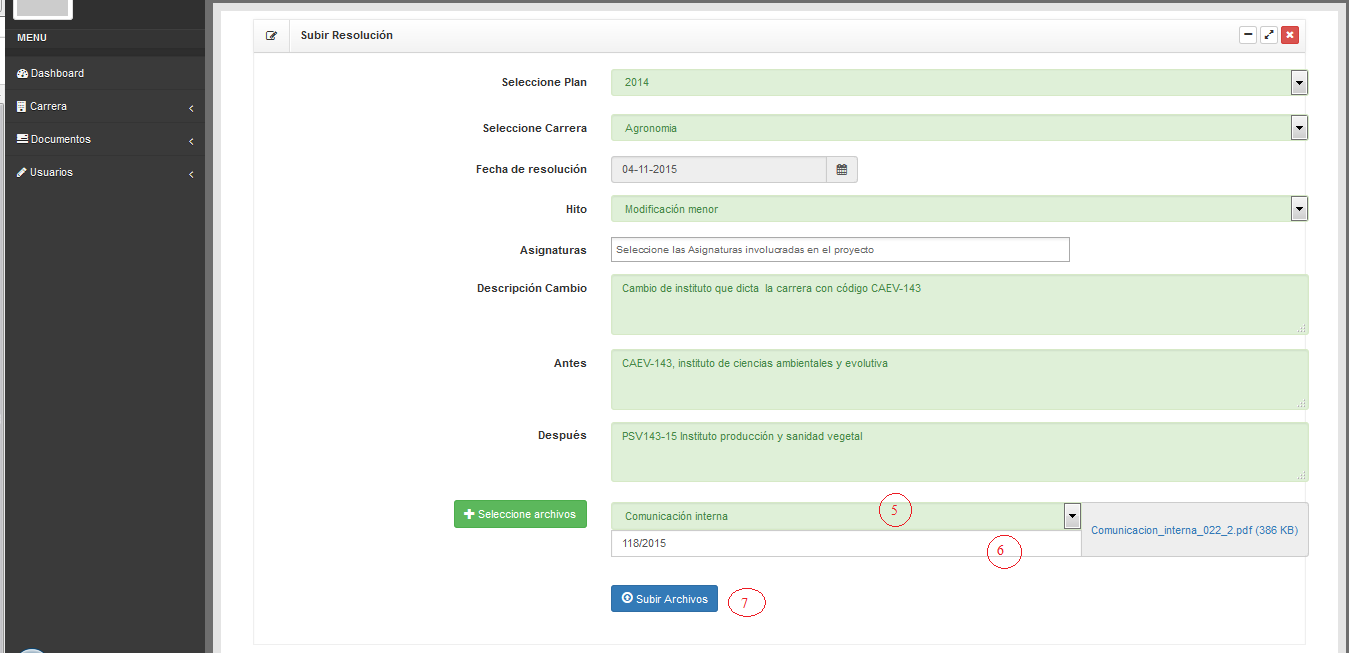
\includegraphics[width=1\textwidth]{images/Capitulo_3/subir_documento5.png}} \\ 
				
				
				\multicolumn{2}{c}{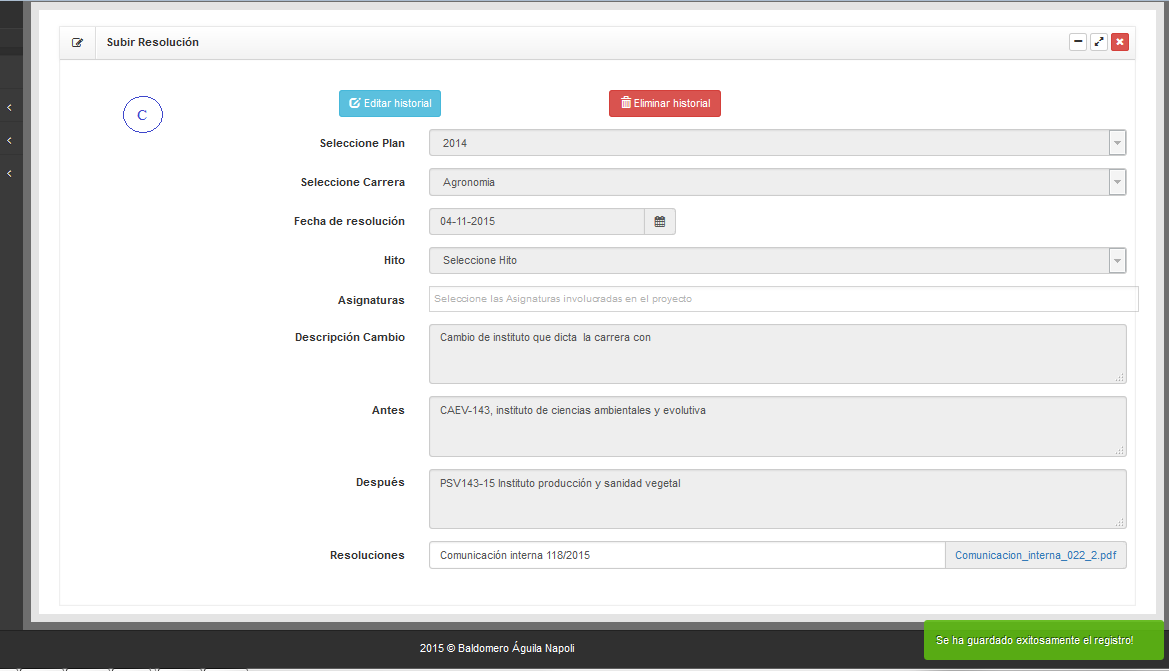
\includegraphics[width=1\textwidth]{images/Capitulo_3/subir_documento6.png}} \\ \hline
				
				\rowcolor{LightBlue2}  \multicolumn{2}{c}{Curso normal de eventos} \\ 
				
				\textbf{Acción actor} &	\textbf{Respuesta sistema} \\ \hline
				
				1.- Este caso de uso comienza cuando un usuario de tipo administrador y/o editor  desea crear un hito curricular, para ello debe hacer click en \textbf{1}.
				&	2.- El sistema despliega la pantalla \textbf{A}, el cual permite al usuario  introducir información referente al encabezado del hito curricular y subir documentos en formato pdf.\\ \hline
			
			
				3.- El usuario ingresa toda la información relacionada con el encabezado del hito curricular en \textbf{2}.
				& 4.- A medida que el usuario va completando los campos, el sistema va validando si están en el formato correcto, es decir, si la información debe ser del tipo: número, sólo letras, longitud máxima, longitud mínima, etc.\\ \hline
				
				5.- Una vez que el usuario haya introducido todos los campos requeridos por el sistema, procede a subir el o los documentos relacionados al hito, haciendo click en \textit{3}.
				& 6.- El sistema abre la ventana que se muestra en \textit{B}.\\ \hline
				
				7.- El usuario selecciona todos los archivos en formato pdf que desee subir, luego hace click en ``Abrir''.
				& 8.- Por cada documento que el usuario desee subir, el sistema  agregará a la interfaz gráfica los siguientes elementos; un DropDownList, en el cual el usuario selecciona el  tipo de documento qué es; un input, donde el usuario ingresa el número del documento y por último un Label que indica el nombre del documento.\\ \hline
				
				9.- El usuario completa los dos campos nuevos que se agregaron a la interfaz gráfica, para luego hacer clik en ``Subir Archivos''.
				& 10.- El sistema valida que los archivos estén en formato correcto.\\ \hline
				
			
				& 11.- El sistema recibe los datos del formulario y los almacena en la base de datos.\\ \hline
				
				& 12.- El sistema almacena la operación que se realizó (En este caso creación de un hito) en la bitácora de cambios del sistema. \\ \hline
				
				& 13.- El sistema redirecciona al usuario a la pantalla \textbf{C}. \\ \hline
				
				\rowcolor{LightBlue2}  \multicolumn{2}{c}{Curso alternativo de los eventos} \\ 
				
			
				& 10.- los archivos que el usuario intenta subir no están en formato pdf, o pesan más de 5 mb, por lo que el sistema muestra un mensaje de alerta y el usuario tiene que volver a la etapa Número 5.\\ \hline
				
			\end{longtable}
			
			


			
			En la Figura \ref{diagrama_secuencial_Subir_documento} se presenta el diagrama de secuencia para este mismo caso de uso, y así mostrar la interacción entre los distintos componentes del software que llevan a cabo esta tarea, a continuación se explicará el diagrama presentado.
			\begin{figure}[H]
				\centering
				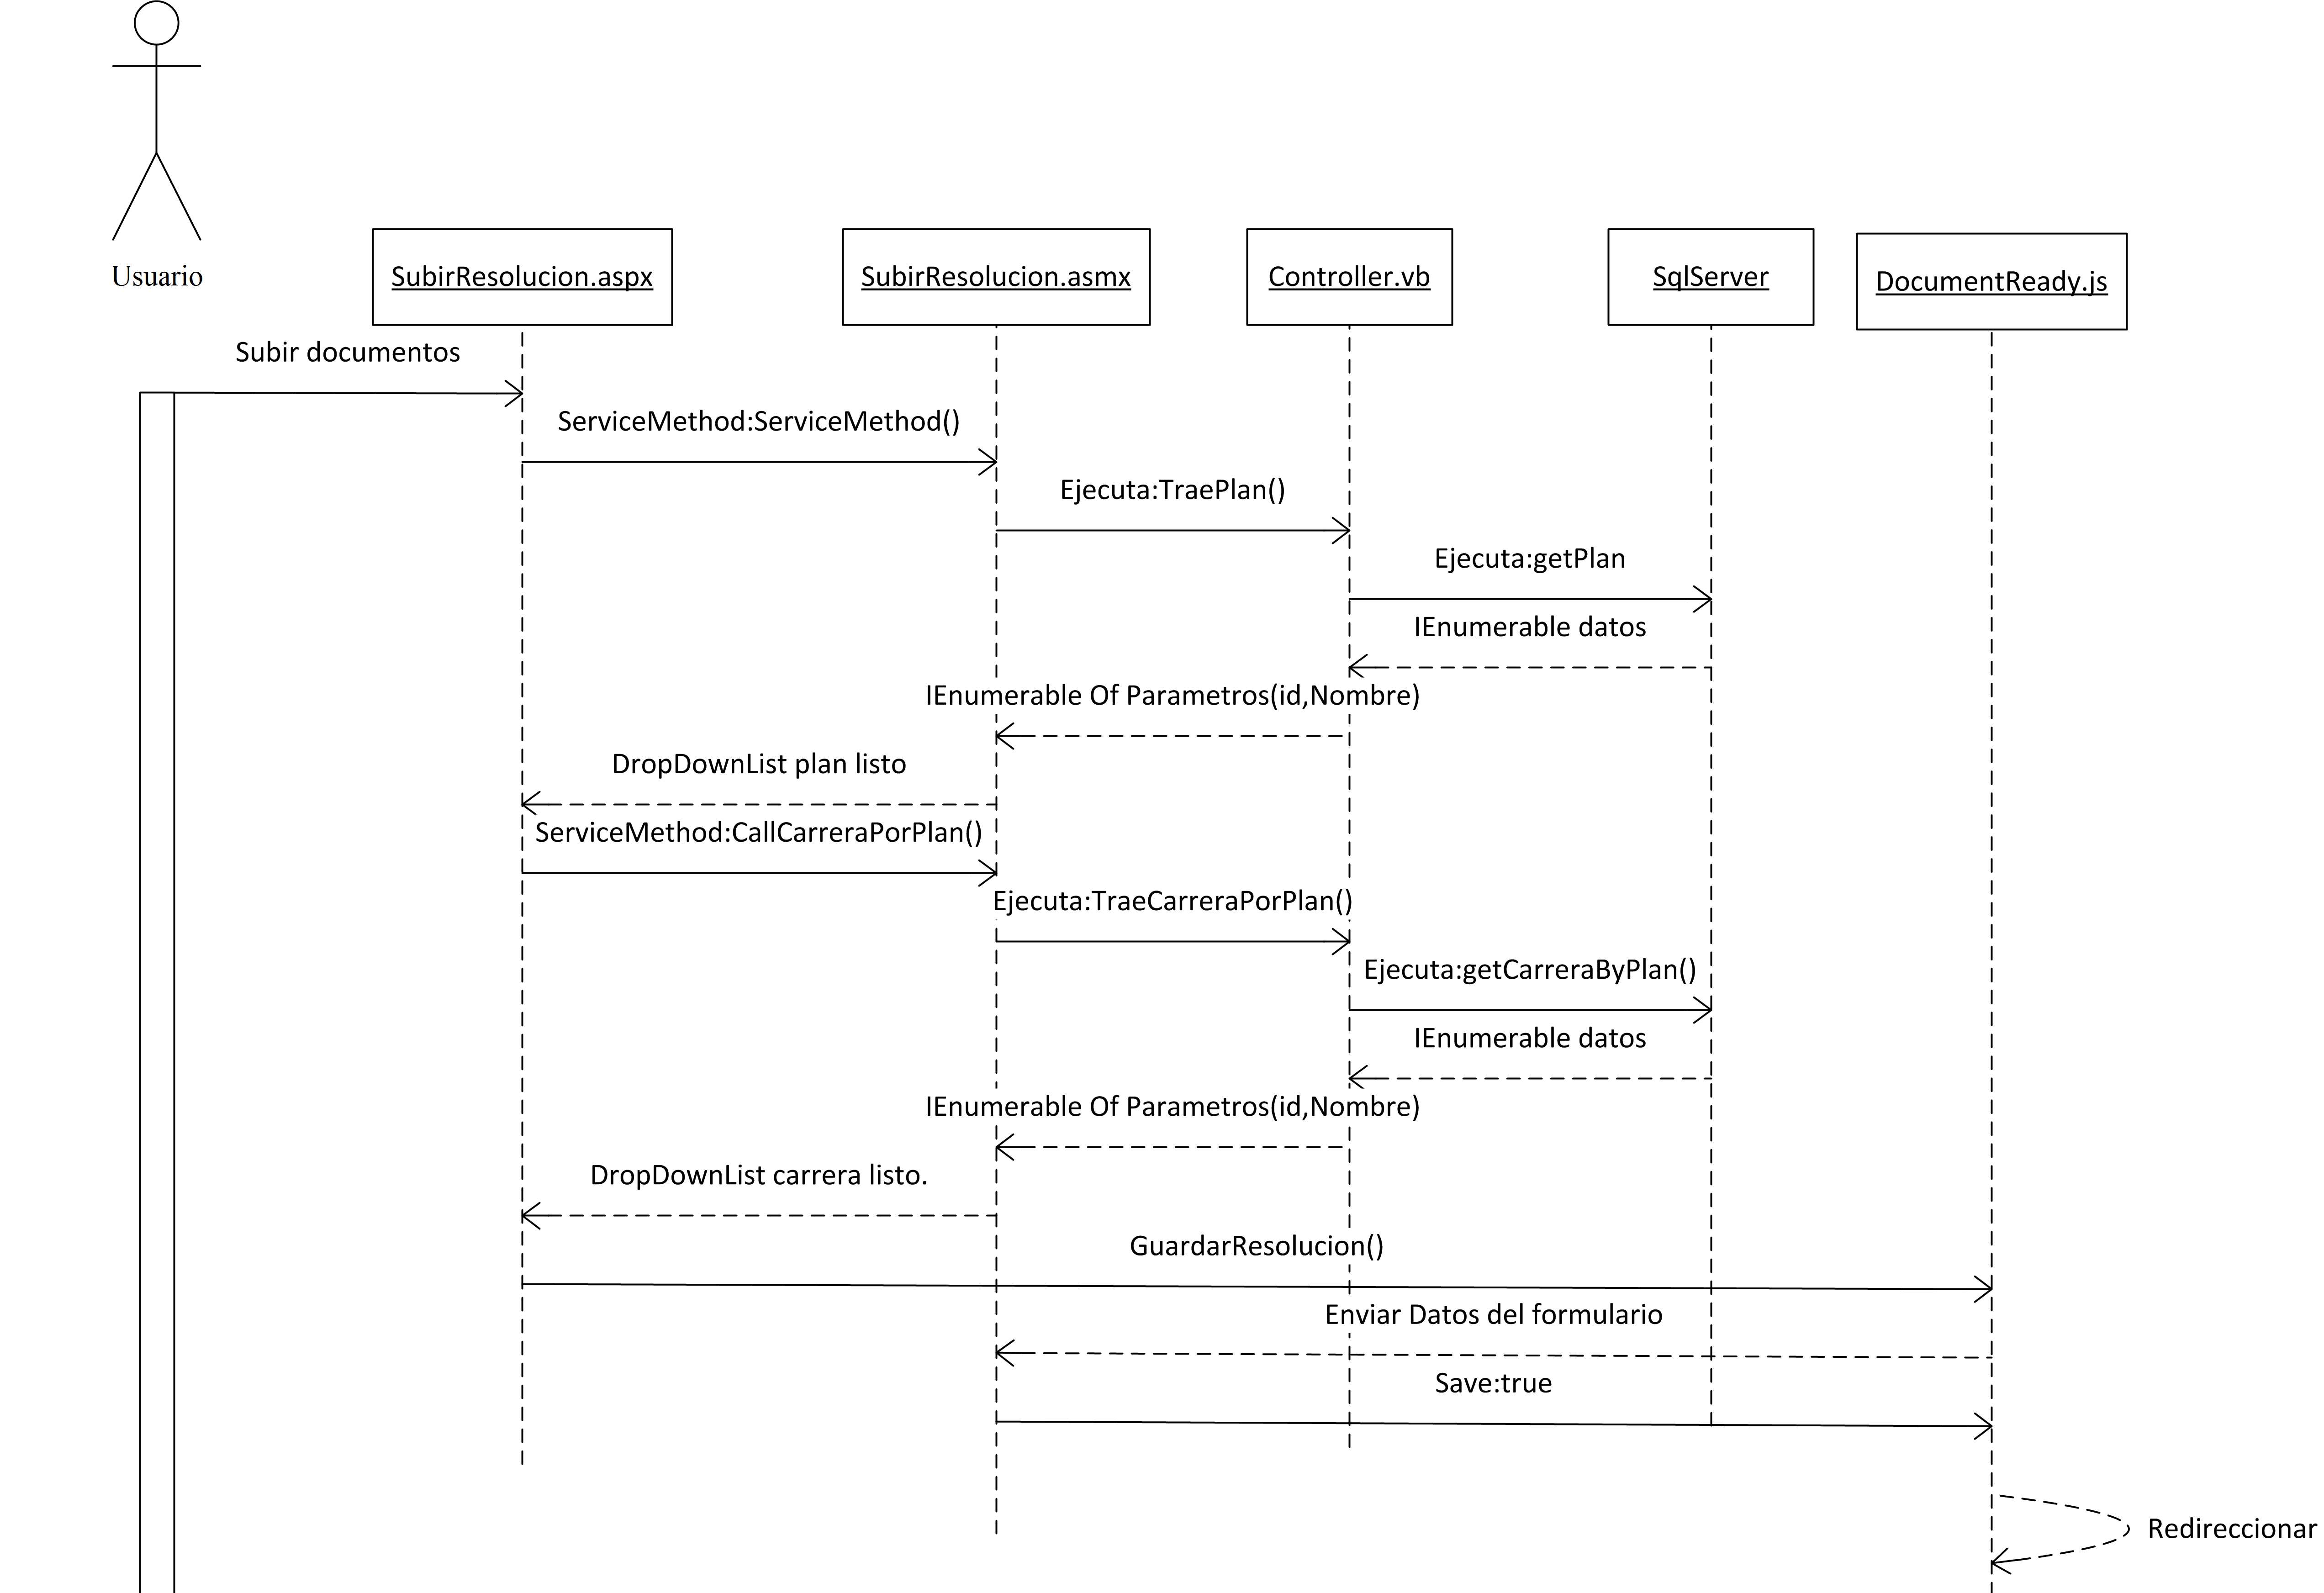
\includegraphics[width=1\textwidth]{images/Capitulo_3/Subir_Documentos.png}
				\caption[Diagrama de secuencia para el caso de uso \textit{Subir Documentos}]{Diagrama de secuencia para el caso de uso \textit{Subir Documentos} \footnote{}}
				\label{diagrama_secuencial_Subir_documento}
			\end{figure}
			\footnotetext{Elaboración propia.}
	
	
	Antes de describir el flujo de control de este caso de uso, hay que mencionar que el módulo Gestor de Documentos trabaja el poblado de los DropDownList del mismo modo que el módulo Historial Curricular, por lo que este proceso no se explicará  con mayor detalle en este diagrama.\\
	
	El flujo de este caso de uso comienza con la carga de la vista SubirResolución.aspx, para ello, antes de mostrar la vista al usuario que realizó la petición, se debe cargar previamente los elementos de las listas  desplegables correspondientes a: planes de estudios y asignaturas. Una vez   \textbf{probada las   listas  desplegables}( ver Sección \ref{Proceso_poblado_DDL} ) el sistema despliega el formulario para que el usuario lo manipule.\\
	
	Luego de que el usuario hay completado los campos necesarios, y haya seleccionado todos los archivos relacionados con el hito curricular que se desea crear, el usuario envía el mensaje \textbf{GuardarResolución} al componente DocumentReady.js, quien es el encargado de  enviar los datos del formulario mediante una petición POST al servicio web \textbf{SubirResolucion.asmx}.\\
	
	El flujo termina cuando el servicio web envía la variable Sabe:true al DocumentReady.js, con el fin de avisarle a este agente de que los cambios se almacenaron correctamente y que puede redireccionar al usuario a la vista de administración de los hitos curriculares.

	
	

	
	
	\mysubparagraph{ Caso de uso real del módulo gestor de documentos:``Ver documentos''} 
	
	El caso de uso ``Ver documentos'' corresponde al segundo caso de uso extendido del caso de uso  ``Gestor de Documentos''. en este caso de uso  todo usuario autentificado tiene acceso y ocurre cuando un  algún usuario quiere ver el repositorio de documentos que se encuentra en el sistema. El caso de uso real se presenta en la Tabla  \ref{Tabla_Caso_Uso_Ver_Documento}.
	
	\begin{longtable}{p{7cm}| p{7cm}}
		
		\caption{Caso de uso  Ver documentos}
		\label{Tabla_Caso_Uso_Ver_Documento}\\
		
		
		\hline
		\endfirsthead
		\multicolumn{2}{c}%
		{\tablename\ \thetable\ -- \textit{Continuación de la página anterior}} \\
		\hline
		
		\hline
		\endhead
		\hline \multicolumn{2}{r}{\textit{Continúa en la página siguiente}} \\
		\endfoot
		\hline \hline
		\endlastfoot
		\rowcolor{LightBlue2}  \multicolumn{2}{c}{Caso de uso  Ver documentos} \\  \hline
		
		
		\textbf{Actores} & Administrador, Editor y Suscriptor.\\ \hline
		
		\textbf{Propósito} & Visualizar el repositorio de documentos de los cambios curriculares de los planes de estudio.\\ \hline
		
		\textbf{Tipo} & Secundario y esencial\\ \hline
		
		\multicolumn{2}{p{15cm}}{\textbf{Resumen:} El administrador, editor o analista selecciona la sección correspondiente a  ver documentos, una vez seleccionado, el sistema  mostrará una tabla con todos los documentos de todas las facultades de la universidad. El usuario tendrá opciones de filtros para buscar ya sea por facultad, escuela, carrera y/o tipo de modificación.} \\  \hline \hline
		
		\rowcolor{LightBlue2}  \multicolumn{2}{c}{Interfaz: Formulario Ver Historial Curricular} \\  \hline \hline
		
		\multicolumn{2}{c}{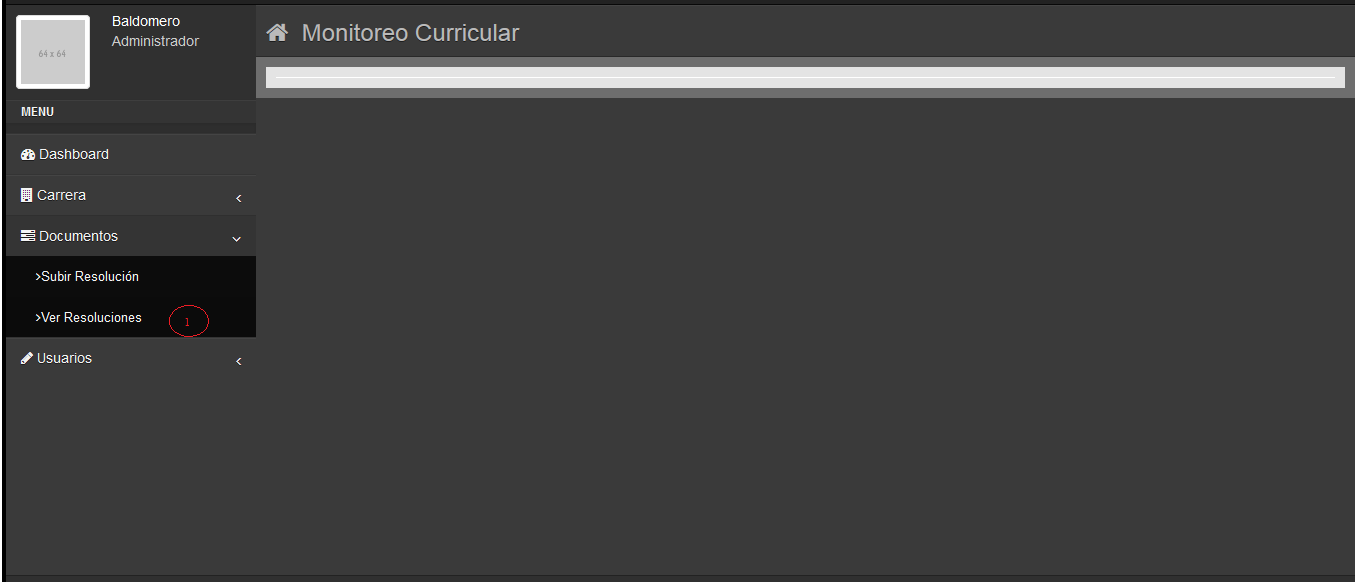
\includegraphics[width=1\textwidth]{images/Capitulo_3/VerDocumentos1.png}} \\ 
		
		\multicolumn{2}{c}{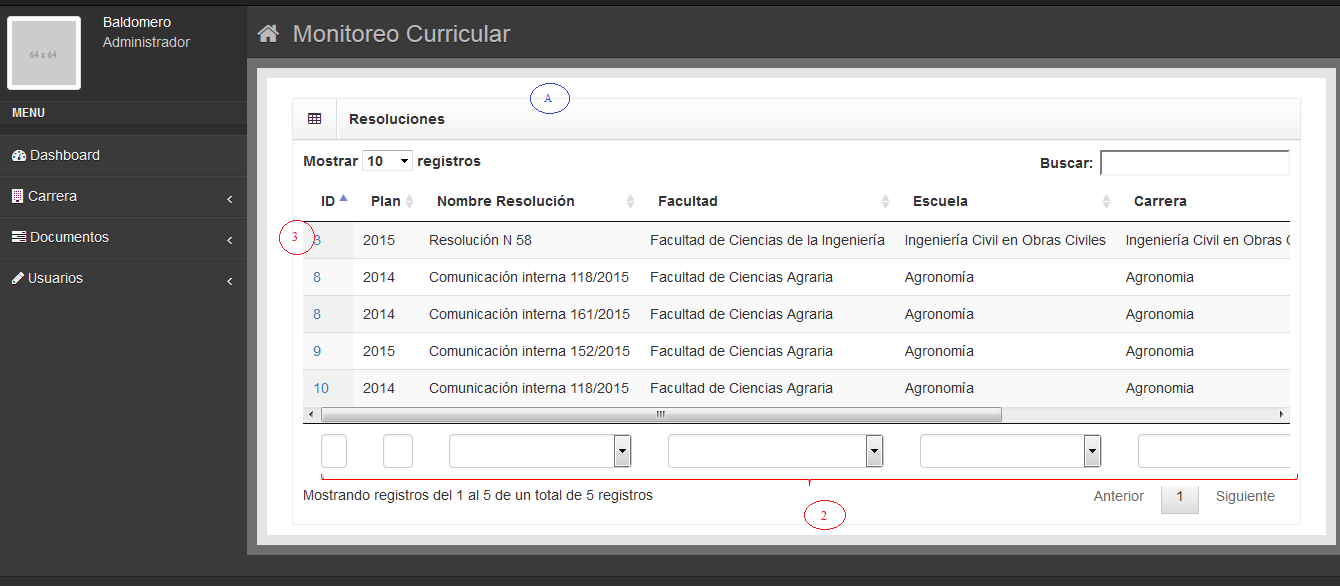
\includegraphics[width=1\textwidth]{images/Capitulo_3/VerDocumentos2.png}} \\ 
		
		\multicolumn{2}{c}{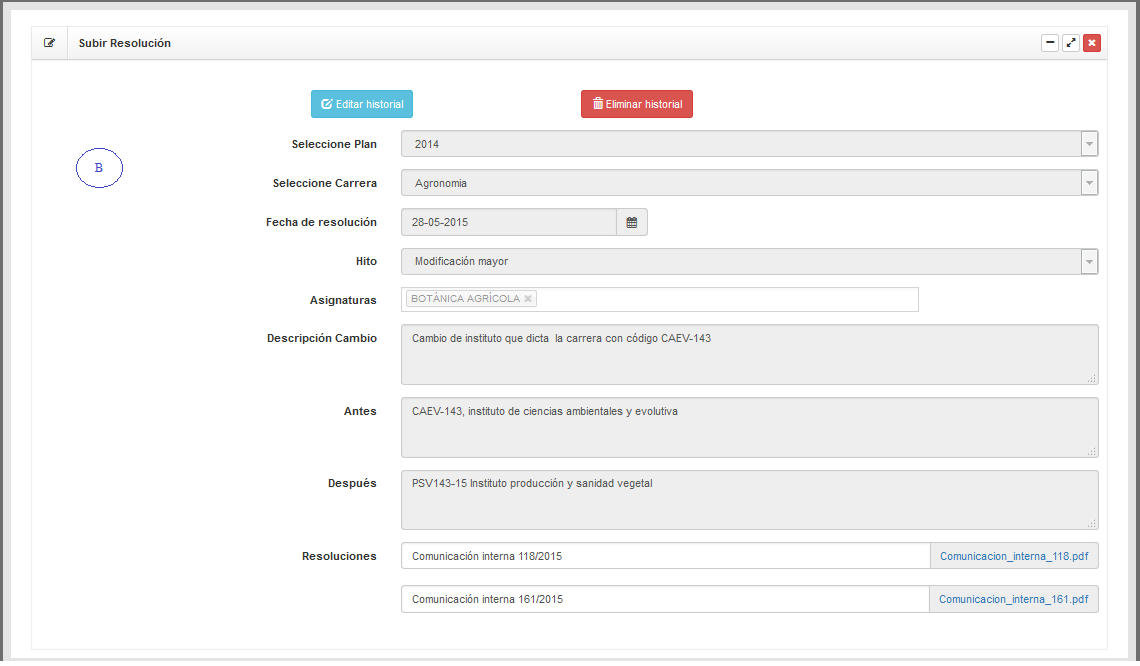
\includegraphics[width=1\textwidth]{images/Capitulo_3/VerDocumentos3.png}} \\  \hline
		
		\rowcolor{LightBlue2}  \multicolumn{2}{c}{Curso normal de eventos} \\ 
		
		\textbf{Acción actor} &	\textbf{Respuesta sistema} \\ \hline
		
		1.- Este caso de uso comienza cuando un usuario autentificado desea ver el repositorio de documentos, para ello debe hacer click en \textbf{1}.
		&	2.- El sistema despliega la pantalla \textbf{A}, el cual permite al usuario visualizar una tabla con el registro de los documentos.\\ \hline
		
		
		3.- El usuario puede hacer algún tipo de filtro avanzado utilizando los DropDownList que se muestran en \textbf{2}.
		& 4.- El complemento DataTable se  encarga de leer los filtros y reducir las filas de la tabla.\\ \hline
		
		5.- El usuario selecciona el hito que desea visualizar, para ello hace click en el id del registro( \textit{3}).
		& 6.- El sistema despliega el hito  con sus documentos en  la ventana que se muestra en \textit{B}.\\ \hline

	
	\end{longtable}
	
	
	
			En la Figura \ref{diagrama_secuencial_ver_documento} se presenta el diagrama de secuencia para este mismo caso de uso, y así mostrar la interacción entre los distintos componentes del software que llevan a cabo esta tarea, a continuación se explicará el diagrama presentado.
			\begin{figure}[H]
				\centering
				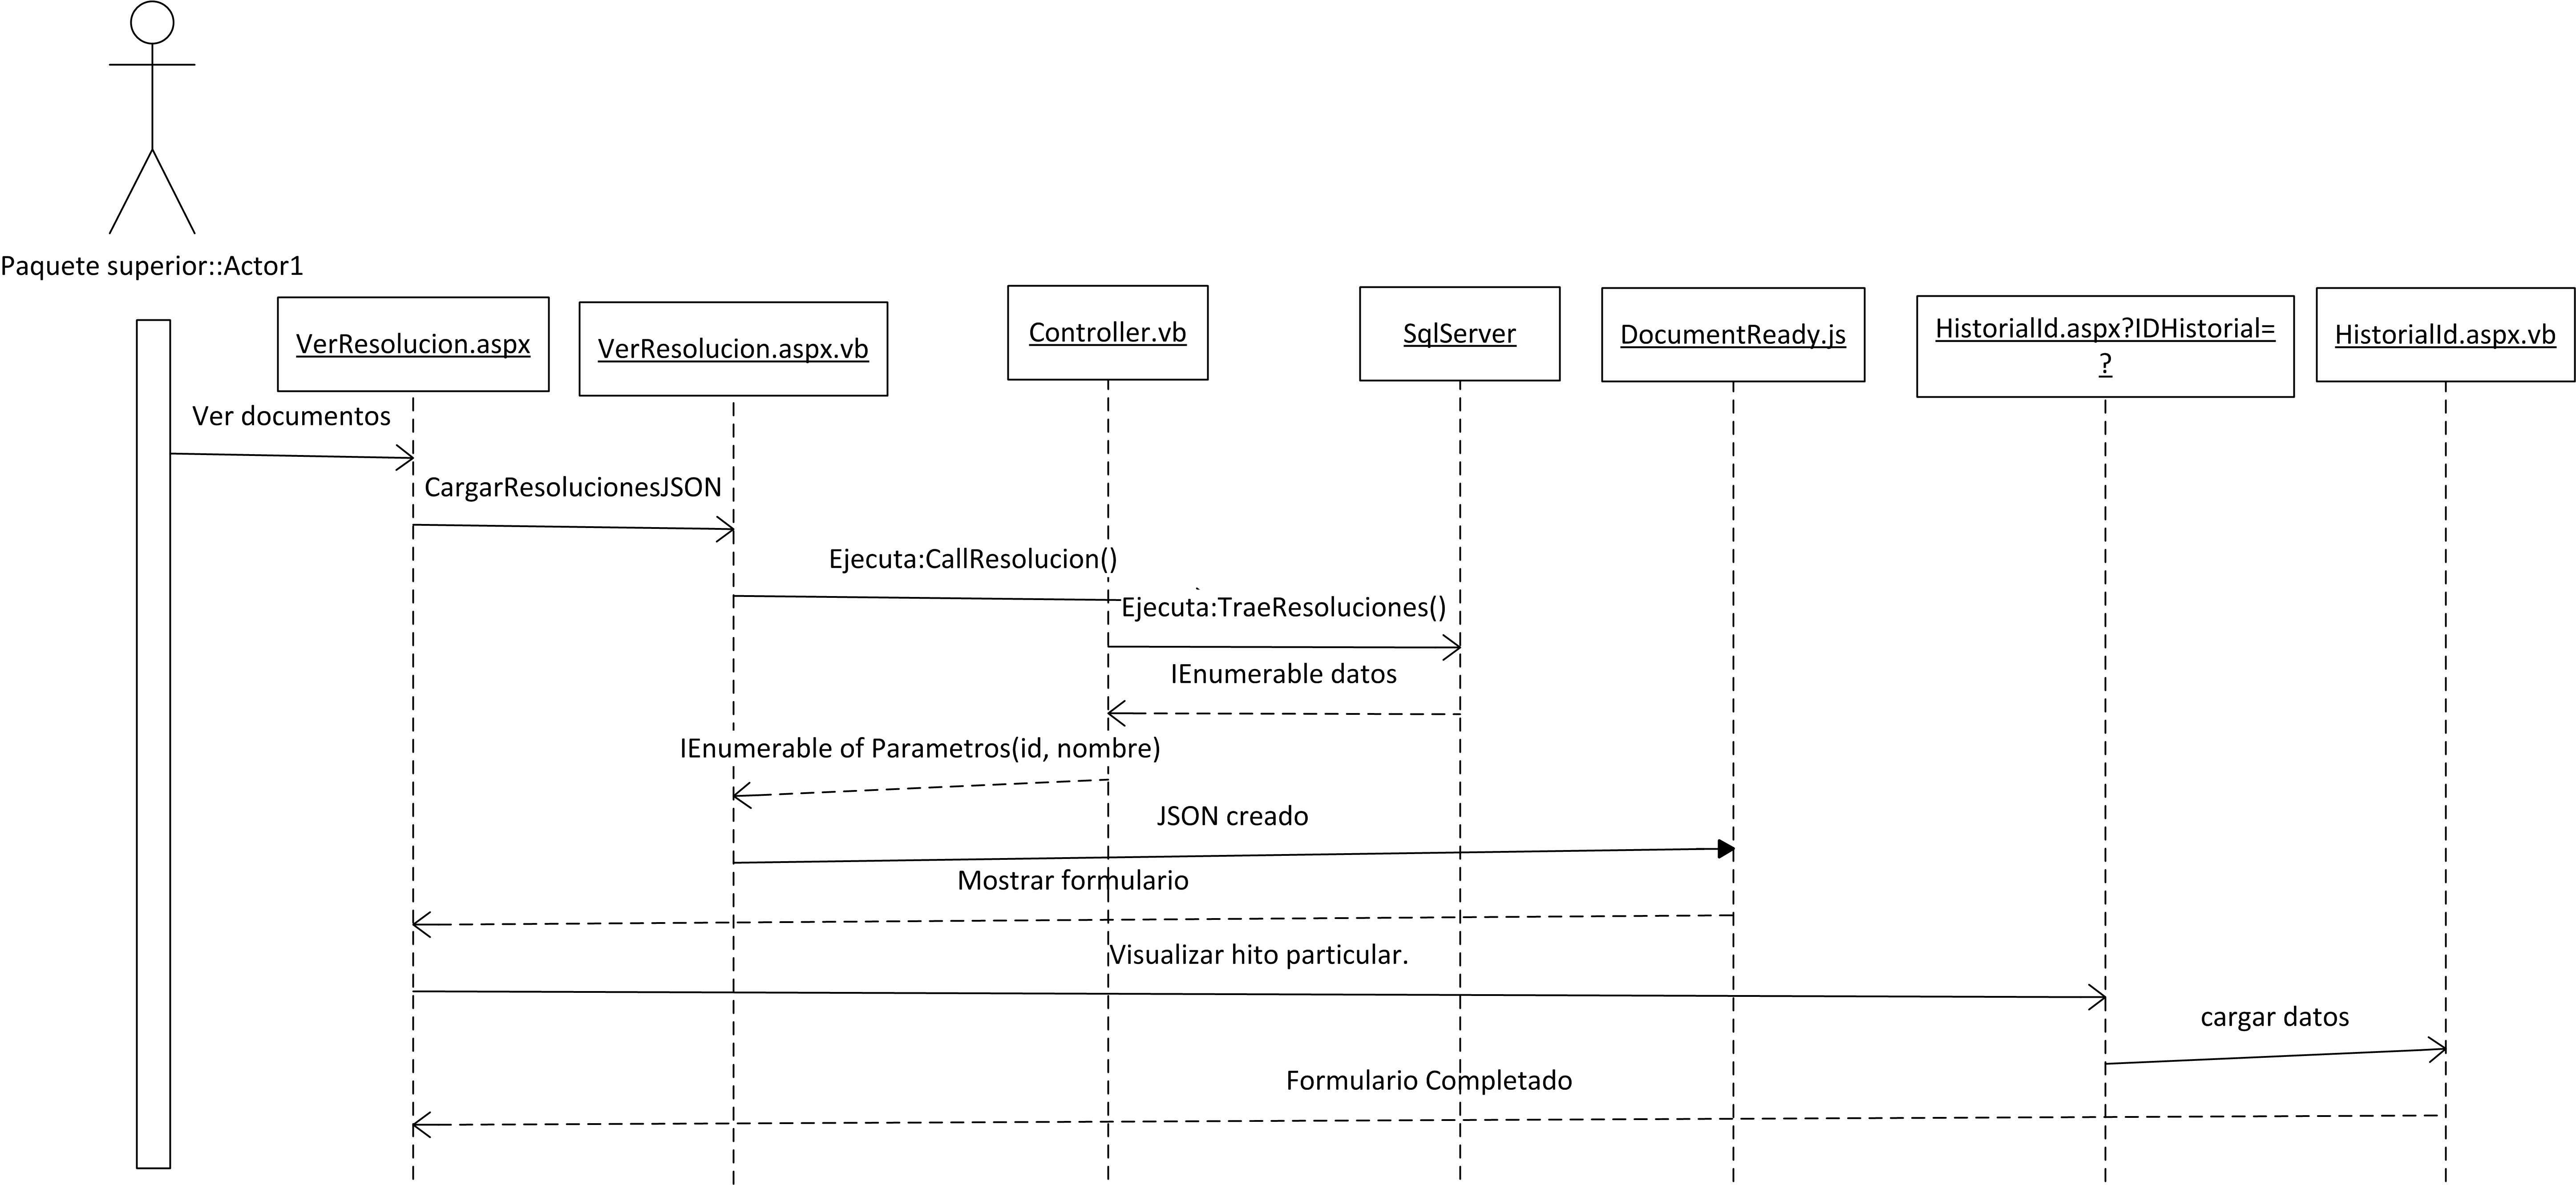
\includegraphics[width=1\textwidth]{images/Capitulo_3/ver_Documentos.png}
				\caption[Diagrama de secuencia para el caso de uso \textit{Ver Documentos}]{Diagrama de secuencia para el caso de uso \textit{Ver Documentos} \footnote{}}
				\label{diagrama_secuencial_ver_documento}
			\end{figure}
			\footnotetext{Elaboración propia.}
			

	Cuando un usuario autentificado desea ver algún documento almacenado en la base de datos (resolución, comunicación interna, decretos, etc.), la vista VerResolucion.aspx es la que comienza con toda la secuencia que permite que este caso de uso se ejecute satisfactoriamente.
	\\
	
	El primero lugar VerResolucion.aspx solicita los datos de todas las resoluciones a la biblioteca Controller.vb mediante la acción CallResolucion(), una vez que esta biblioteca reciba el mensaje, ejecuta el procedimiento almacenado TraeResoluciones().
	\\
	
	Una vez que la consulta se haya efectuado exitosamente, la biblioteca Controller tiene que dar formato a estos  datos obtenidos de la base de datos, para que posteriormente se envíen al \textit{code behind} \footnote{Archivo que contiene el código ejecutable de las vistas en ASP.NET} de la vista VerResolucion.aspx.
	\\
	
	Después de que la vista VerResolucion.aspx reciba los datos del Controller.vb, crea el Archivo JSON y se envía una variable JSON = true al agente DocumentReady.js. Al recibir la variable de éxito, DocumentReady.js se encarga de cargar los datos del archivo a la tabla y finalmente mostrar formulario final al usuario autentificado.






